\documentclass{bmstu}

\usepackage{amsmath}

% Для листинга кода:
\lstset{ %
	language=Sql,   					% выбор языка для подсветки	
	basicstyle=\small\sffamily,			% размер и начертание шрифта для подсветки кода
	numbers=left,						% где поставить нумерацию строк (слева\справа)
	%numberstyle=,					% размер шрифта для номеров строк
	stepnumber=1,						% размер шага между двумя номерами строк
	numbersep=5pt,						% как далеко отстоят номера строк от подсвечиваемого кода
	frame=single,						% рисовать рамку вокруг кода
	tabsize=4,							% размер табуляции по умолчанию равен 4 пробелам
	captionpos=t,						% позиция заголовка вверху [t] или внизу [b]
	breaklines=true,					
	breakatwhitespace=true,				% переносить строки только если есть пробел
	escapeinside={\#*}{*)},				% если нужно добавить комментарии в коде
	backgroundcolor=\color{white},
         literate={а}{{\selectfont\char224}}1
          {б}{{\selectfont\char225}}1
          {в}{{\selectfont\char226}}1
          {г}{{\selectfont\char227}}1
          {д}{{\selectfont\char228}}1
          {е}{{\selectfont\char229}}1
          {ё}{{\"e}}1
          {ж}{{\selectfont\char230}}1
          {з}{{\selectfont\char231}}1
          {и}{{\selectfont\char232}}1
          {й}{{\selectfont\char233}}1
          {к}{{\selectfont\char234}}1
          {л}{{\selectfont\char235}}1
          {м}{{\selectfont\char236}}1
          {н}{{\selectfont\char237}}1
          {о}{{\selectfont\char238}}1
          {п}{{\selectfont\char239}}1
          {р}{{\selectfont\char240}}1
          {с}{{\selectfont\char241}}1
          {т}{{\selectfont\char242}}1
          {у}{{\selectfont\char243}}1
          {ф}{{\selectfont\char244}}1
          {х}{{\selectfont\char245}}1
          {ц}{{\selectfont\char246}}1
          {ч}{{\selectfont\char247}}1
          {ш}{{\selectfont\char248}}1
          {щ}{{\selectfont\char249}}1
          {ъ}{{\selectfont\char250}}1
          {ы}{{\selectfont\char251}}1
          {ь}{{\selectfont\char252}}1
          {э}{{\selectfont\char253}}1
          {ю}{{\selectfont\char254}}1
          {я}{{\selectfont\char255}}1
          {А}{{\selectfont\char192}}1
          {Б}{{\selectfont\char193}}1
          {В}{{\selectfont\char194}}1
          {Г}{{\selectfont\char195}}1
          {Д}{{\selectfont\char196}}1
          {Е}{{\selectfont\char197}}1
          {Ё}{{\"E}}1
          {Ж}{{\selectfont\char198}}1
          {З}{{\selectfont\char199}}1
          {И}{{\selectfont\char200}}1
          {Й}{{\selectfont\char201}}1
          {К}{{\selectfont\char202}}1
          {Л}{{\selectfont\char203}}1
          {М}{{\selectfont\char204}}1
          {Н}{{\selectfont\char205}}1
          {О}{{\selectfont\char206}}1
          {П}{{\selectfont\char207}}1
          {Р}{{\selectfont\char208}}1
          {С}{{\selectfont\char209}}1
          {Т}{{\selectfont\char210}}1
          {У}{{\selectfont\char211}}1
          {Ф}{{\selectfont\char212}}1
          {Х}{{\selectfont\char213}}1
          {Ц}{{\selectfont\char214}}1
          {Ч}{{\selectfont\char215}}1
          {Ш}{{\selectfont\char216}}1
          {Щ}{{\selectfont\char217}}1
          {Ъ}{{\selectfont\char218}}1
          {Ы}{{\selectfont\char219}}1
          {Ь}{{\selectfont\char220}}1
          {Э}{{\selectfont\char221}}1
          {Ю}{{\selectfont\char222}}1
          {Я}{{\selectfont\char223}}1
          {λ}{{\selectfont\char955}}1
 }

\bibliography{biblio}

\begin{document}

% \makecourseworktitle{}{}{}{}{}{}{}{}

% ***************************************************************************


\maketableofcontents

% ****************************************************************************
\chapter*{ВВЕДЕНИЕ}
\addcontentsline{toc}{chapter}{ВВЕДЕНИЕ}

Одной из важнейших задач обеспечения безопасности взаимодействия процессов в распределенных системах является задача контроля входящего трафика на определенный хост.

Возможным методом контроля является динамическое обнаружение атак. 

Для решения задачи обнаружения атак во входящем трафике используется специальное программное обеспечение, которое может быть реализовано в виде загружаемого модуля ядра для ОС Linux.

Разработке такого программного обеспечения посвящена данная работа.


\chapter{Аналитический раздел}
\section{Постановка задачи}
В соответствии с заданием на курсовую работу необходимо разработать загружаемый модуль ядра для ОС Linux, осуществляющий динамическое обнаружение атак во входящем сетевом трафике. 

% Предусмотреть возможность сокрытия разработанного загружаемого модуля ядра для ОС Linux.

% Для взаимодействия с разработанным модулем ядра для ОС Linux разработать отдельное программное обеспечение (ПО).

Для достижения поставленной задачи необходимо:
\begin{itemize}
	\item[---] провести анализ принципов работы сетевой подсистемы ОС Linux;
	\item[---] провести анализ способов перехвата сетевых пакетов;
	% \item провести анализ программного интерфейса, который предоставляет ОС Linux для работы с сетевыми пакетами;
        \item[---] провести анализ методов динамического обнаружения атак;
	\item[---] разработать алгоритм и стороннее ПО для выявления атак в сетевом трафике;
	\item[---] предусмотреть возможность сокрытия разработанного загружаемого модуля ядра для ОС Linux.
\end{itemize}

\section{Сетевая модель OSI}
В распределённых системах информация передаётся в виде пакетов по протоколам. Передаваемые данные подвергаются процессам инкапсуляции и декапсуляции, в процессе которых каждый пакет проходит все уровни сетевой модели OSI (таблица \ref{osi_table}).

\begin{table}[h]
	\begin{center}
		\caption{Модель OSI}
		\label{osi_table}
		\begin{tabular}{| p{1cm} | p{7cm} |}
			\hline
			\textbf{№} 	& \textbf{Название} \\
			\hline
			7 		& Прикладной уровень\\ 
			\hline
			6 		& Уровень представления  \\ 
			\hline
			5 		& Сеансовый уровень \\ 
			\hline
			4 		& Транспортный уровень \\ 
			\hline
			3 		& Сетевой уровень \\ 
			\hline
			2 		& Канальный уровень \\ 
			\hline
			1 		& Физический уровень \\ 
			\hline
		\end{tabular}
	\end{center}
\end{table}

\section*{Internet Protocol}

Internet Protocol (IP) --- протокол сетевого уровня модели OSI.

Данный протокол объединяет сегменты сети в единую сеть, обеспечивая доставку пакетов данных между любыми узлами сети через произвольное число промежуточных узлов (маршрутизаторов). Именно поэтому он стал тем протоколом, который объединил отдельные компьютерные сети во всемирную сеть Интернет. 

IP не гарантирует надёжной доставки пакета до адресата --- в частности, пакеты могут прийти не в том порядке, в котором были отправлены, продублироваться (приходят две копии одного пакета), оказаться повреждёнными (обычно повреждённые пакеты уничтожаются) или не прийти вовсе.

На рисунке \ref{img:ip_header} представлен заголовок пакета IPv4.
\begin{figure}[hbtp]
 \centering
 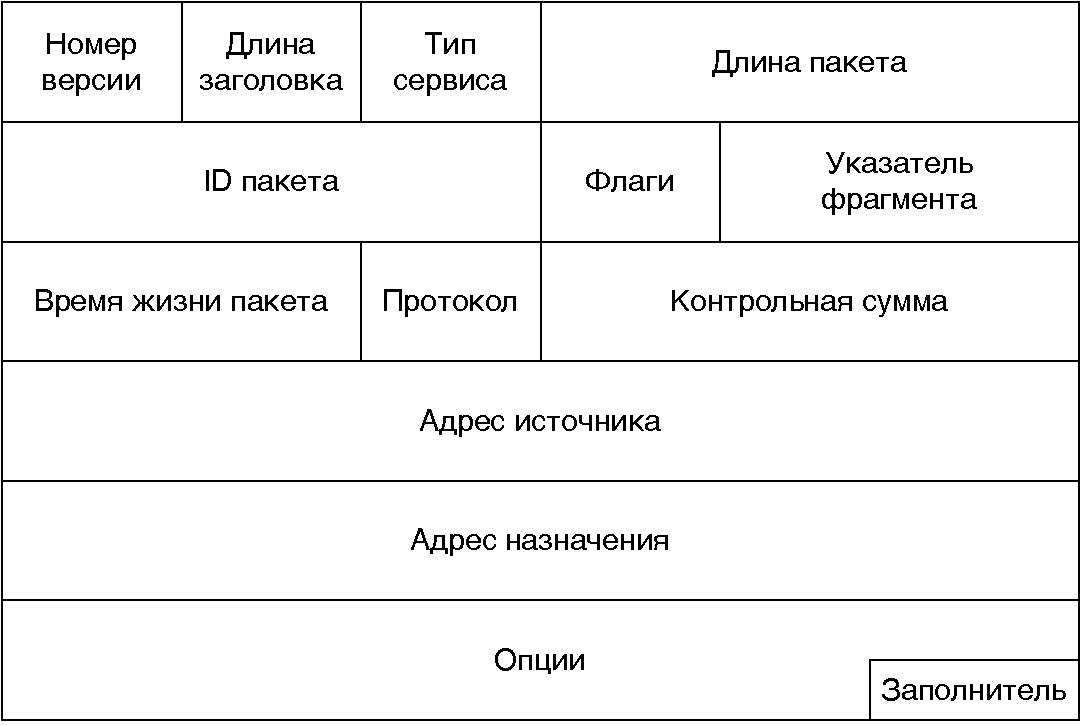
\includegraphics[width=0.6\textwidth]{inc/img/ip_header.pdf}
 \caption{Заголовок пакета IP}
 \label{img:ip_header}
\end{figure}

\section*{Transmission Control Protocol}
Transmission Control Protocol (TCP) --- протокол транспортного уровня модели OSI.

Механизм TCP предоставляет поток данных с предварительной установкой соединения, осуществляет повторный запрос данных в случае потери данных и устраняет дублирование при получении двух копий одного пакета, гарантируя тем самым (в отличие от UDP) целостность передаваемых данных и уведомление отправителя о результатах передачи.

На рисунке \ref{img:tcp_header} представлен заголовок сегмента TCP.
\begin{figure}[hbtp]
 \centering
 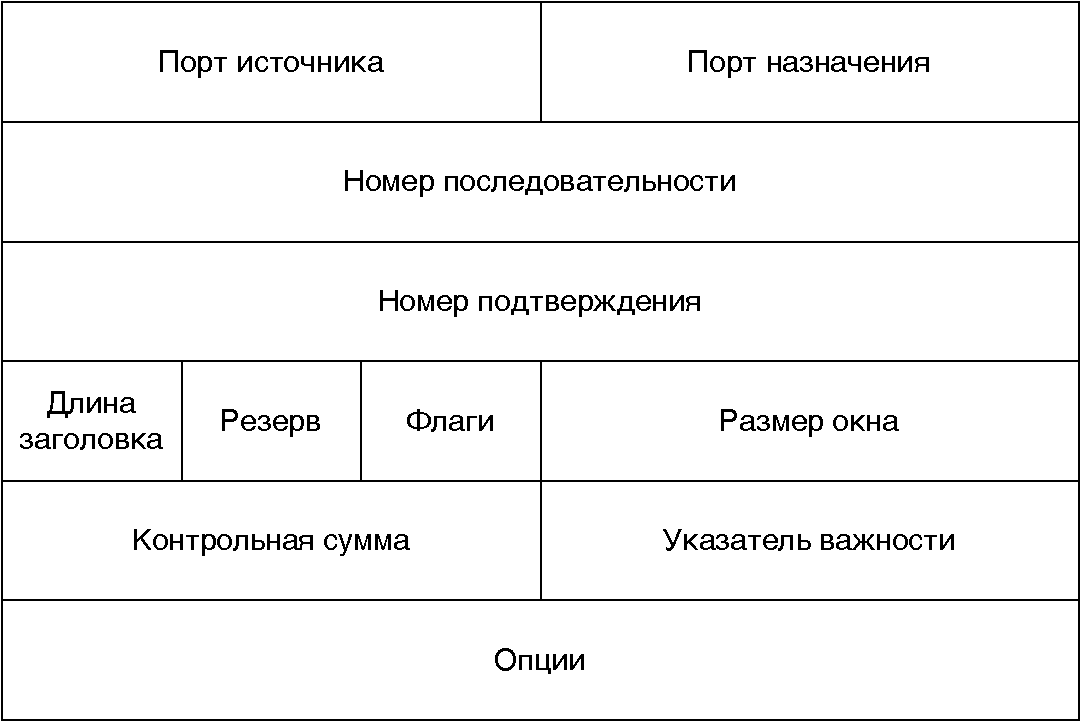
\includegraphics[width=0.6\textwidth]{inc/img/tcp_header.pdf}
 \caption{Заголовок пакета TCP}
 \label{img:tcp_header}
\end{figure}

\textbf{Флаги:}
\begin{itemize}
    \item[---] \textbf{URG} --- поле <<указатель важности>> имеет смысл;
    \item[---] \textbf{ACK} --- данный сегмент является подтверждением получения предыдущего;
    \item[---] \textbf{PSH} --- нужно передать немедленно;
    \item[---] \textbf{RST} --- аварийное закрытие соединения;
    \item[---] \textbf{SYN} --- открытие соединения;
    \item[---] \textbf{FIN} --- корректное завершение соединения.
\end{itemize}

% Чтобы установить надежное соединение, TCP использует процесс, называемый термином \textbf{<<трехстороннее рукопожатие>>} (TCP three-way/triple handshake).

% \textbf{Установление соединения TCP} --- трехстороннее рукопожатие (квитирование). 

% Для установления соединения между сервером и клиентом используется \textbf{трехстороннее рукопожатие} (квитирование). Это трехэтапный процесс, который требует, чтобы клиент и сервер обменялись пакетами синхронизации и подтверждения, прежде чем начнется обмен данными.

\textbf{Трехстороннее рукопожатие TCP} --- это процесс, который устанавливает соединение между клиентом и сервером. Он состоит из трех этапов, где каждая сторона обменивается определенными пакетами синхронизации и подтверждения, чтобы убедиться, что обе стороны готовы к обмену данными.

\begin{enumerate}
    \item Клиент отправляет серверу пакет синхронизации (SYN), чтобы начать установку соединения.
    \item Сервер получает пакет SYN, затем отправляет пакет синхронизации и подтверждения (SYN-ACK) клиенту, указывая, что он готов к установлению соединения.
    \item Клиент затем отправляет серверу пакет подтверждения (ACK), завершая процесс установки соединения.
\end{enumerate}
% 1. Клиент отправляет серверу пакет синхронизации (SYN), чтобы начать установку соединения.
% 2. Сервер получает пакет SYN, затем отправляет пакет синхронизации и подтверждения (SYN-ACK) клиенту, указывая, что он готов к установлению соединения.
% 3. Клиент затем отправляет серверу пакет подтверждения (ACK), завершая процесс установки соединения.

Принцип выполнения трехстороннего рукопожатия TCP представлен на рисунке \ref{img:tcp_receipt}.

\begin{figure}[hbtp]
 \centering
 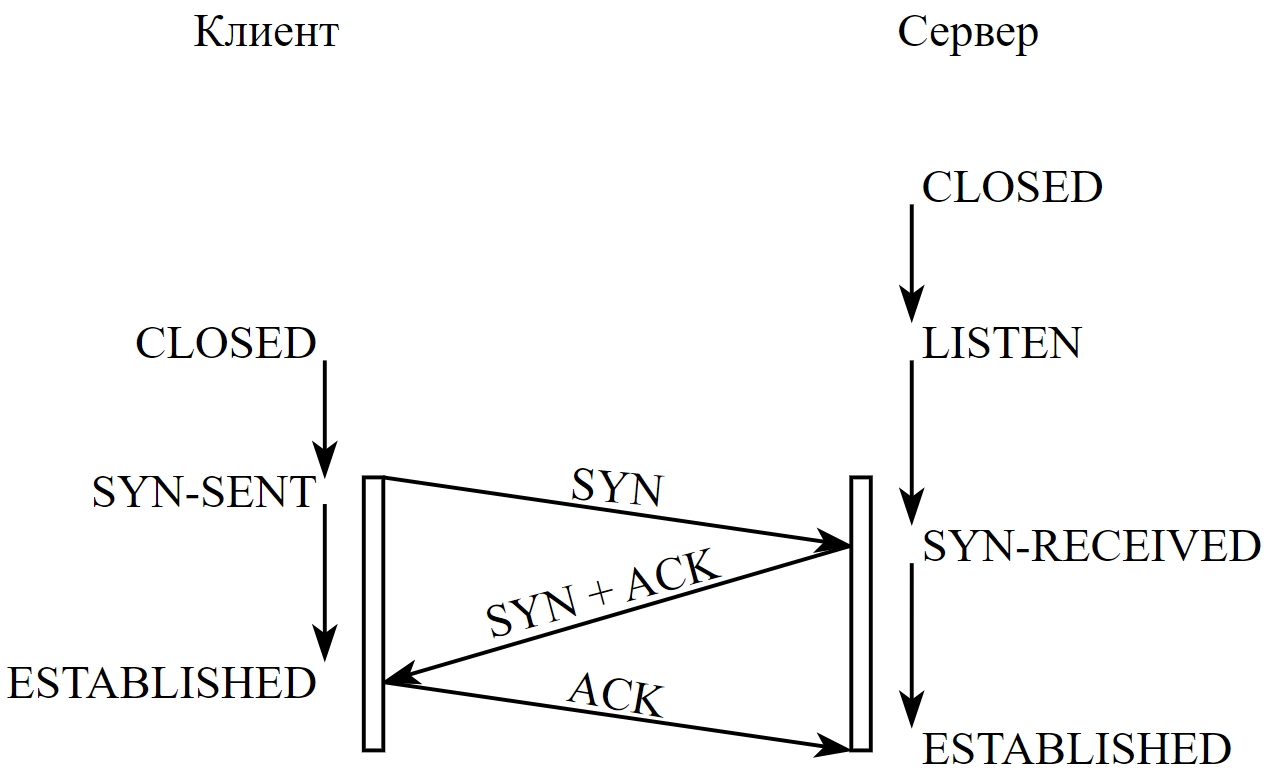
\includegraphics[width=0.8\textwidth]{inc/img/3way.png}
 \caption{Установление соединения TCP}
 \label{img:tcp_receipt}
\end{figure}

% \newpage


\section{Удаленная сетевая атака}

\textbf{Удалённая сетевая атака} --- информационное разрушающее воздействие на распределённую вычислительную систему, осуществляемое программно по каналам связи.

Выдяют следующие виды удаленных сетевых атак.

\begin{enumerate}
    \item По характеру воздействия:
        \begin{itemize}
            \item[---] \textbf{пассивная атака} --- атака не оказывает непосредственное влияние на функционирование системы, но может нарушить ее политику безопасности. 
            % Подобное воздействие практически невозможно обнаружить. Относятся: анализ трафика, прослушка канала связи;
            \item[---] \textbf{активная атака} --- атака оказывает непосредственное влияние на работу системы (нарушение работоспособности, искажение или навязывание информации) и нарушающее в ней политику безопасности. 
            
            % Особенностью такого воздействия является принципиально возможное его обнаружение и возможная идентификация его источника.
        \end{itemize}
    \item По цели воздействия:
        \begin{itemize}
            \item[---] нарушение конфиденциальности информации или параметров системы;
            \item[---] нарушение целостности информации;
            \item[---] нарушение работоспособности или доступности компонент системы.
        \end{itemize}
    \item По условию начала воздействия:
        \begin{itemize}
            \item[---] \textbf{атака по запросу} от атакуемого объекта --- атакующая сторона ожидает от потенциальной цели атаки запроса определенного типа, который будет условием начала воздействия;
            \item[---] \textbf{атака по наступлению ожидаемого события} на атакуемом объекте;
            \item[---] \textbf{безусловная атака} --- осуществляется независимо от состояния и работоспособности объекта.
        \end{itemize}
    \item По наличию обратной связи с атакуемом объектом:
        \begin{itemize}
            \item[---] \textbf{с операционной системой} --- между атакующим узлом и жертвой существует операционная система, которая позволяет атакующему адекватно реагировать на все изменения, происходящие на стороне жертвы;
            \item[---] \textbf{без операционной системы} или однонаправленная атака.
        \end{itemize}
    \item По расположению субъекта атаки относительно жертвы:
        \begin{itemize}
            \item[---] \textbf{внутрисегментное} --- находится в одной подсети;
            \item[---] \textbf{межсегментное или удаленное} --- взаимодействие осуществляется через промежуточные узы или маршрутизаторы.
        \end{itemize}
    \item По уровню модели OSI, на который осуществляется воздействие.
\end{enumerate}

Примерами атак на сетевом уровне являются: перекрытие пакетов, IP Spoofing (подмена IP), ARP Spoofing, затопление ICMP пакетами.

Примеры атак на транспортном уровне: ранняя десинхронизация, локальная буря, затопление SYN пакетами (SYN flood).

\section*{DDoS-атака}

\textbf{Denial of Service (DoS)} --- хакерская атака на вычислительную систему с целью довести её до отказа, то есть создание таких условий, при которых добросовестные пользователи системы не смогут получить доступ к предоставляемым системным ресурсам (серверам), либо этот доступ будет затруднён. Отказ «вражеской» системы может быть и шагом к овладению системой (если в нештатной ситуации ПО выдаёт какую-либо критическую информацию --- например, версию, часть программного кода и так далее). Но чаще это мера экономического давления: потеря простой службы, приносящей доход, счета от провайдера и меры по уходу от атаки ощутимо бьют по карману «цели».


\textbf{Distributed Denial of Service} --- распределенная DoS-атака. Такая атака проводится в том случае, если требуется вызвать отказ в обслуживании хорошо защищённой крупной компании или правительственной организации. 

DDoS-атака обычно состоит из следующих этапов.

\begin{enumerate}
    \item Злоумышленник сканирует крупную сеть с помощью специально подготовленных сценариев, которые выявляют потенциально слабые узлы.
    \item Выбранные узлы подвергаются нападению, и злоумышленник получает на них права администратора.
    \item На захваченные узлы устанавливаются программы, которые работают в фоновом режиме. Теперь эти компьютеры называются компьютерами-зомби, их пользователи даже не подозревают, что являются потенциальными участниками DDoS-атаки.
    \item Злоумышленник отправляет определенные команды захваченным компьютерам и те, в свою очередь осуществляют коллективную DoS-атаку на целевой компьютер.
\end{enumerate}

% Первым делом злоумышленник сканирует крупную сеть с помощью специально подготовленных сценариев, которые выявляют потенциально слабые узлы. 
% Выбранные узлы подвергаются нападению, и злоумышленник получает на них права администратора. На захваченные узлы устанавливаются программы, которые работают в фоновом режиме. Теперь эти компьютеры называются компьютерами-зомби, их пользователи даже не подозревают, что являются потенциальными участниками DDoS-атаки. Далее злоумышленник отправляет определенные команды захваченным компьютерам и те, в свою очередь осуществляют коллективную DoS-атаку на целевой компьютер.

На рисунке \ref{img:ddos} представлен принцип проведения DDoS-атаки.

В настоящее время DoS и DDoS-атаки наиболее популярны, так как позволяют довести до отказа практически любую плохо написанную систему, не оставляя юридически значимых улик.

\begin{figure}[hbtp]
 \centering
 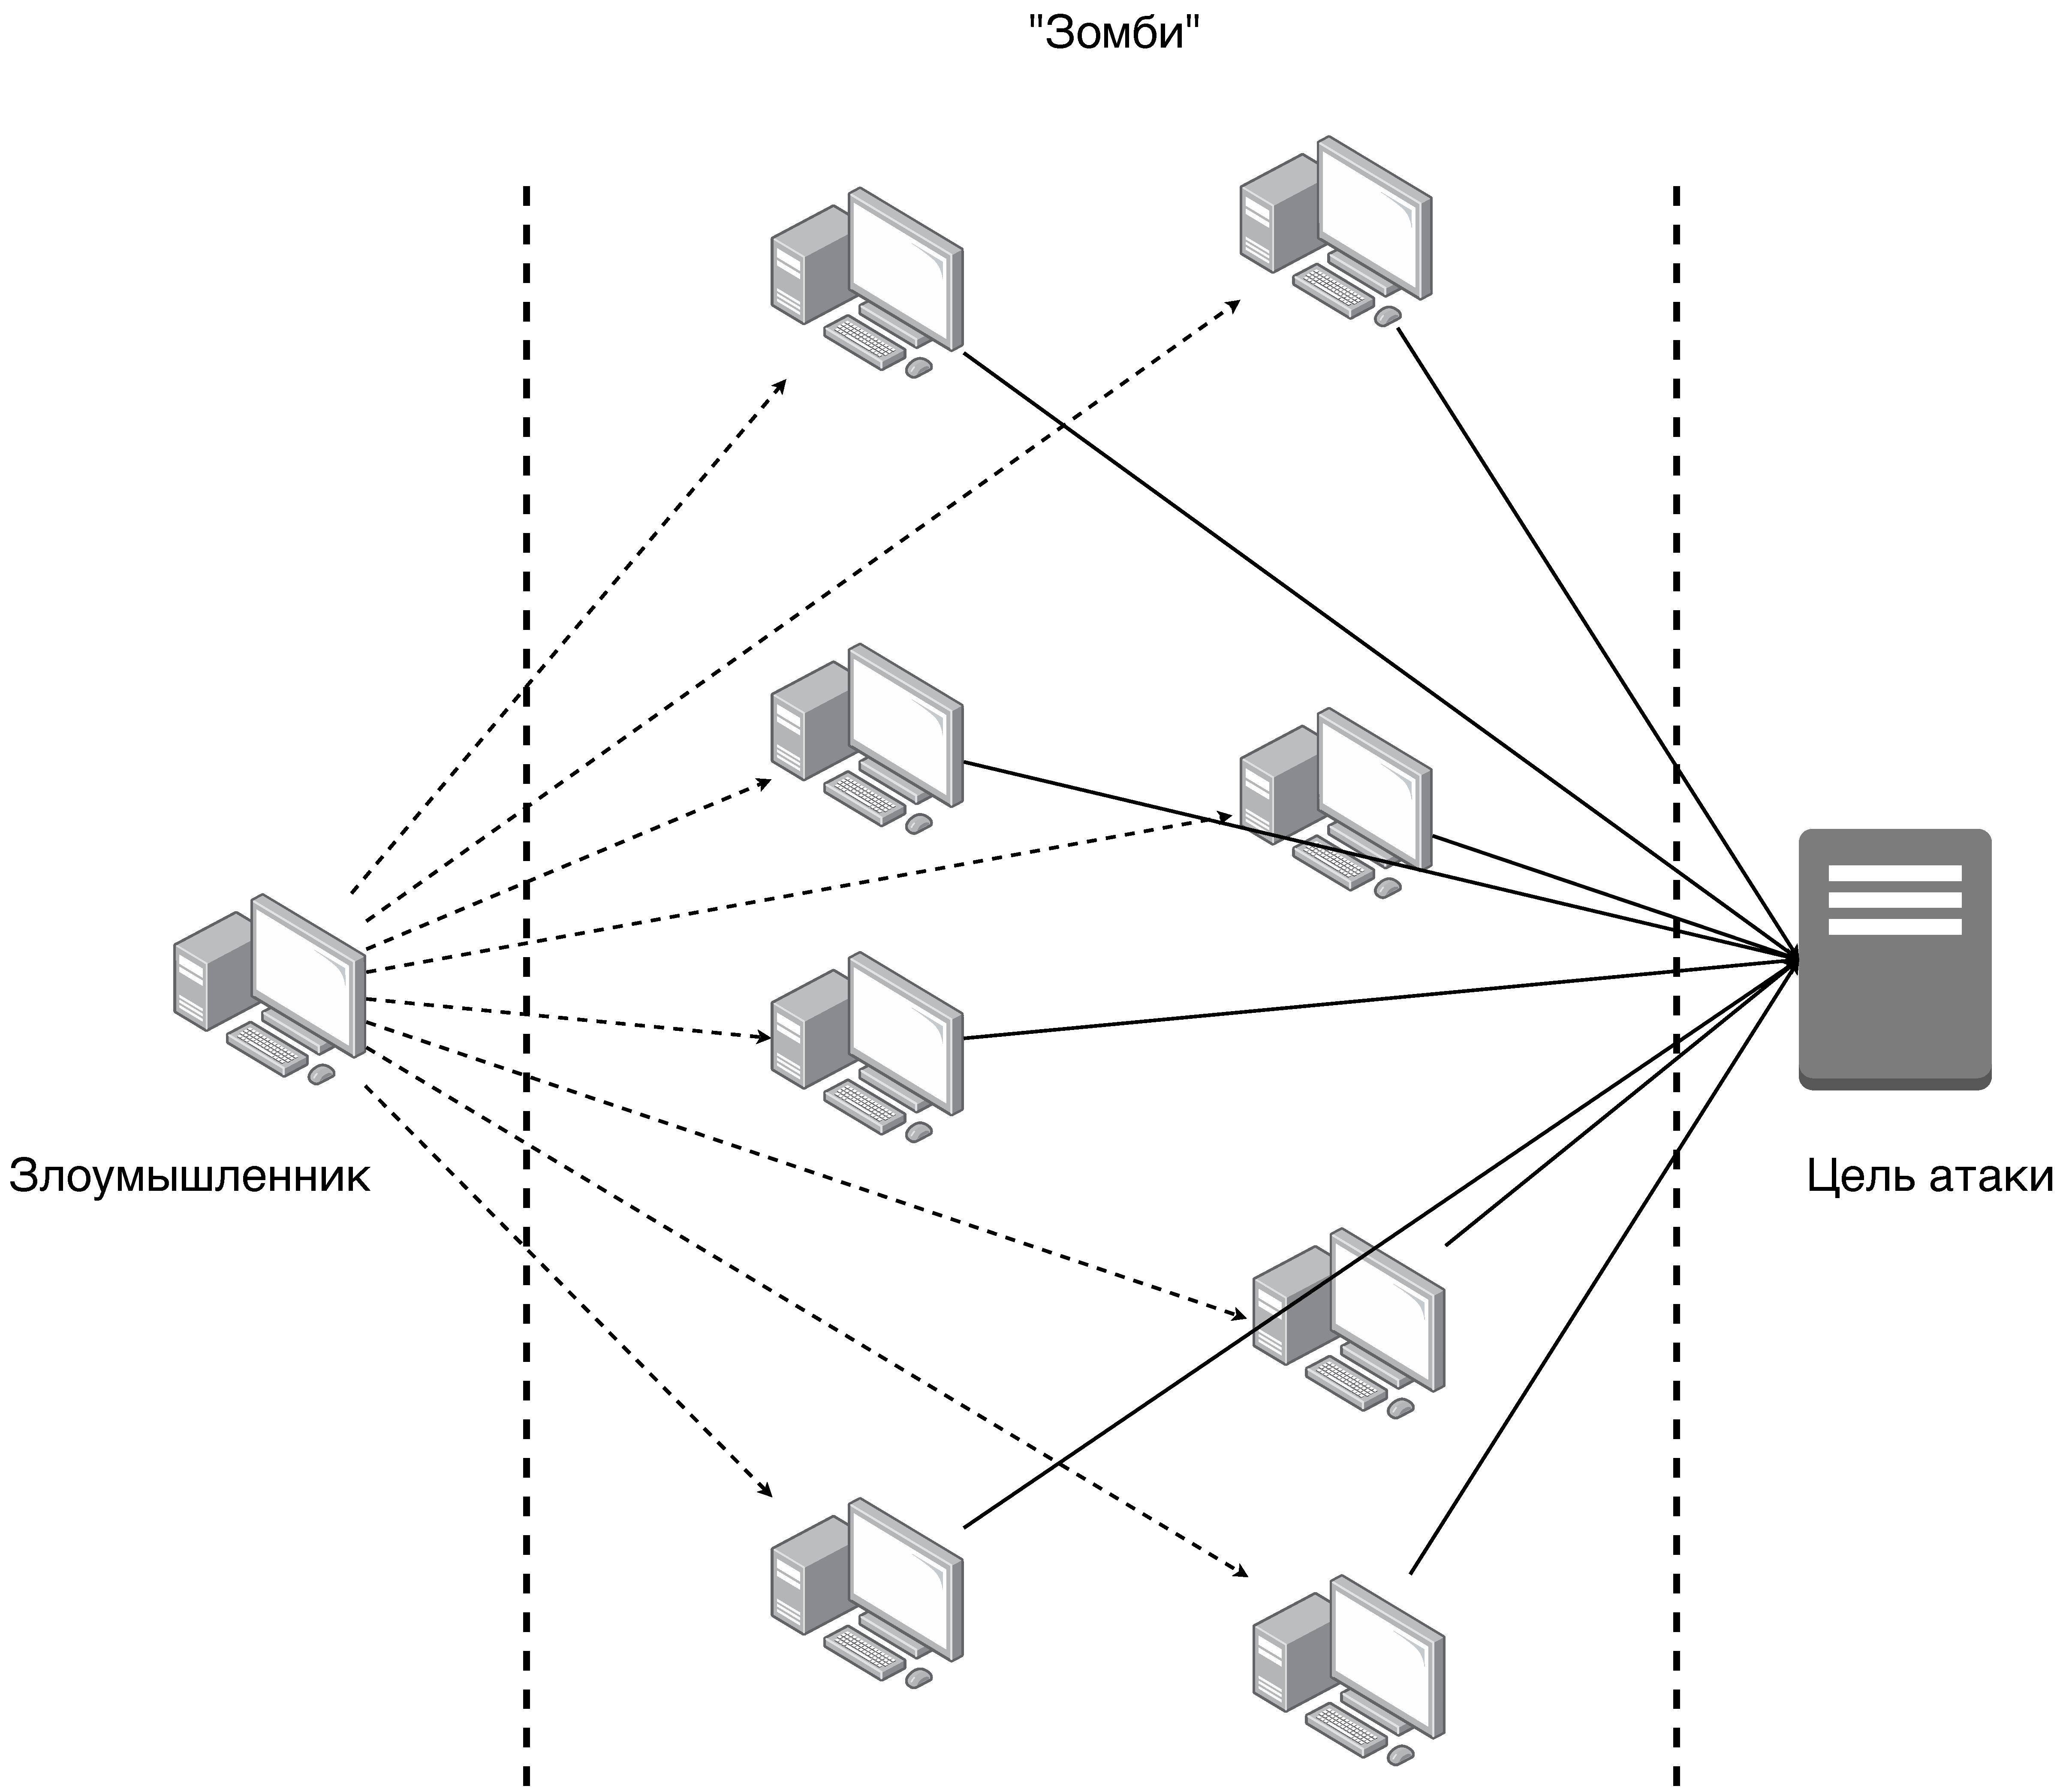
\includegraphics[width=0.78\textwidth]{inc/img/ddos.pdf}
 \caption{DDoS атака}
 \label{img:ddos}
\end{figure}


% \section{Защита от удаленных сетевых атак}

% Для защиты от сетевых атак применяется ряд фильтров, подключенных к интернет-каналу с большой пропускной способностью. Фильтры действуют таким образом, что последовательно анализируют проходящий трафик, выявляя нестандартную сетевую активность и ошибки. В число анализируемых шаблонов нестандартного трафика входят все известные на сегодняшний день методы атак, в том числе реализуемые и при помощи распределённых бот-сетей. Фильтры могут реализовываться как на уровне маршрутизаторов, управляемых свитчей, так и специализированными аппаратными средствами.

\section{Атака SYN-flood}

\textbf{Syn-flood атака} --- это одна из разновидностей DoS-атак. 

Принцип следующий: злоумышленник посылает огромное количество запросов установки соединения на атакуемый сервер. Сервер, видя сегменты с флагом SYN, выделяет необходимые ресурсы для поддержания соединения и отправляет в ответ сегменты с флагами SYN, ACK, переходя в состояние SYN-RECEIVED (такое состояние еще называют полуоткрытым соединением). Злоумышленник, не шлет ответные ACK сегменты, а продолжает бомбардировать сервер SYN-запросами, тем самым вынуждая сервер создавать все больше и больше полуоткрытых соединений. Сервер располагает ограниченными ресурсами, и потому имеет лимит на количество полуоткрытых соединений. Ввиду этой ограниченности, при достижении предельного числа полуоткрытых соединений сервер начинает отклонять новые попытки соединения. Таким образом и достигается отказ в обслуживании (Denial of Service)~\cite{synflood}.



% \section*{Методы предотвращения DDoS-атак}

% Существуют различные методы предотвращения DDoS-атак, включая ограничение скорости, фильтрацию IP-адресов и использование систем предотвращения вторжений (IPS).

% Ограничение скорости предполагает установку лимитов на количество запросов, которые могут быть отправлены с одного IP-адреса за определенный период времени. Это может помочь предотвратить перегрузку системы большим количеством запросов.

% Фильтрация IP-адресов заключается в блокировке трафика от IP-адресов, которые подозреваются в участии в DDoS-атаке. Этот метод может быть эффективным, но он также может привести к блокировке легитимного трафика.

% Системы предотвращения вторжений (IPS) используются для обнаружения и блокировки DDoS-атак на основе анализа паттернов трафика и сигнатур атак.

% Важно отметить, что эффективная защита от DDoS-атак требует комплексного подхода, включающего в себя не только технические меры, но и организационные меры, такие как разработка и внедрение политик безопасности, обучение персонала и регулярное тестирование системы на уязвимости.

\section*{Методы защиты от SYN-flood атак}

Для защиты от SYN-flood атак существует два подхода, которые можно комбинировать между собой.

\begin{enumerate}
    \item Увеличить количество полуоткрытых TCP-соединений и уменьшить время, в котором сокет может пребывать в состоянии SYN-RECEIVED.
    \item Использовать SYN-cookie.
\end{enumerate}

Идея SYN-cookie очень проста: когда к нам приходит SYN-запрос мы не создаем новое соединение, а отправляем SYN, ACK ответ клиенту, где в поле Sequence Number кодируем данные о данном соединении. Если мы получаем ACK ответ от клиента, то из поля Acknowledgment Number восстанавливаем данные о соединении. Данный метод хорош тем, что мы более не будем выделять ресурсы, как только к нам придет SYN-запрос. Но есть и очевидный минус: если наш пакет затеряется, или подвергнется искажению, то мы не сможем отправить его повторно, так как информацию о соединении мы условились не сохранять.


% \section*{Методы обнаружения SYN-flood атак}

% Основной признак SYN-flood атак --- деградация онлайн-сервиса, а также полная или частичная недоступность IT-систем. Анализ трафика помогает обнаружить атаку и по косвенным признакам:    

% \begin{itemize}
%     \item[---] подозрительные скачки объёмов трафика с одного IP-адреса (или диапазона IP-адресов);
%     \item[---] поток трафика от пользователей, имеющих одинаковый поведенческий профиль (тип устройства, геолокация или версия браузера);
%     \item[---] аномальные всплески запросов к одной веб-странице/эндпоинту или в необычное для веб-ресурса время.
% \end{itemize}

% Общий алгоритм выявления сетевых атак может быть описан следующим образом. Данными для анализа является сетевой трафик, представленный как набор сетевых пакетов, в общем случае
% фрагментированных на уровне IP. Собранные сырые данные в дальнейшем послужат источником при формировании необходимой информации для последующего анализа. Так, полученные данные могут
% быть агрегированы за определенный временной интервал и нормализованы с целью задания признаковых атрибутов общего вида, которые
% потребуются при построении текущего профиля активности. Созданный набор признаков сравнивается с набором характеристик нормальной деятельности объекта (пользователя или системы) --- шаблоном
% нормального поведения. Существенное расхождение
% сравниваемых параметров фиксируется. Иначе происходит уточнение шаблона нормального поведения
% посредством изменения параметров его настройки с учетом текущего
% наблюдаемого профиля сетевой активности. 

% На рисунке~\ref{img:clasification} приведена классификация основных методов обнаружения сетевых атак~\cite{браницкий2016анализ}.

% \begin{figure}[hbtp]
%  \centering
%  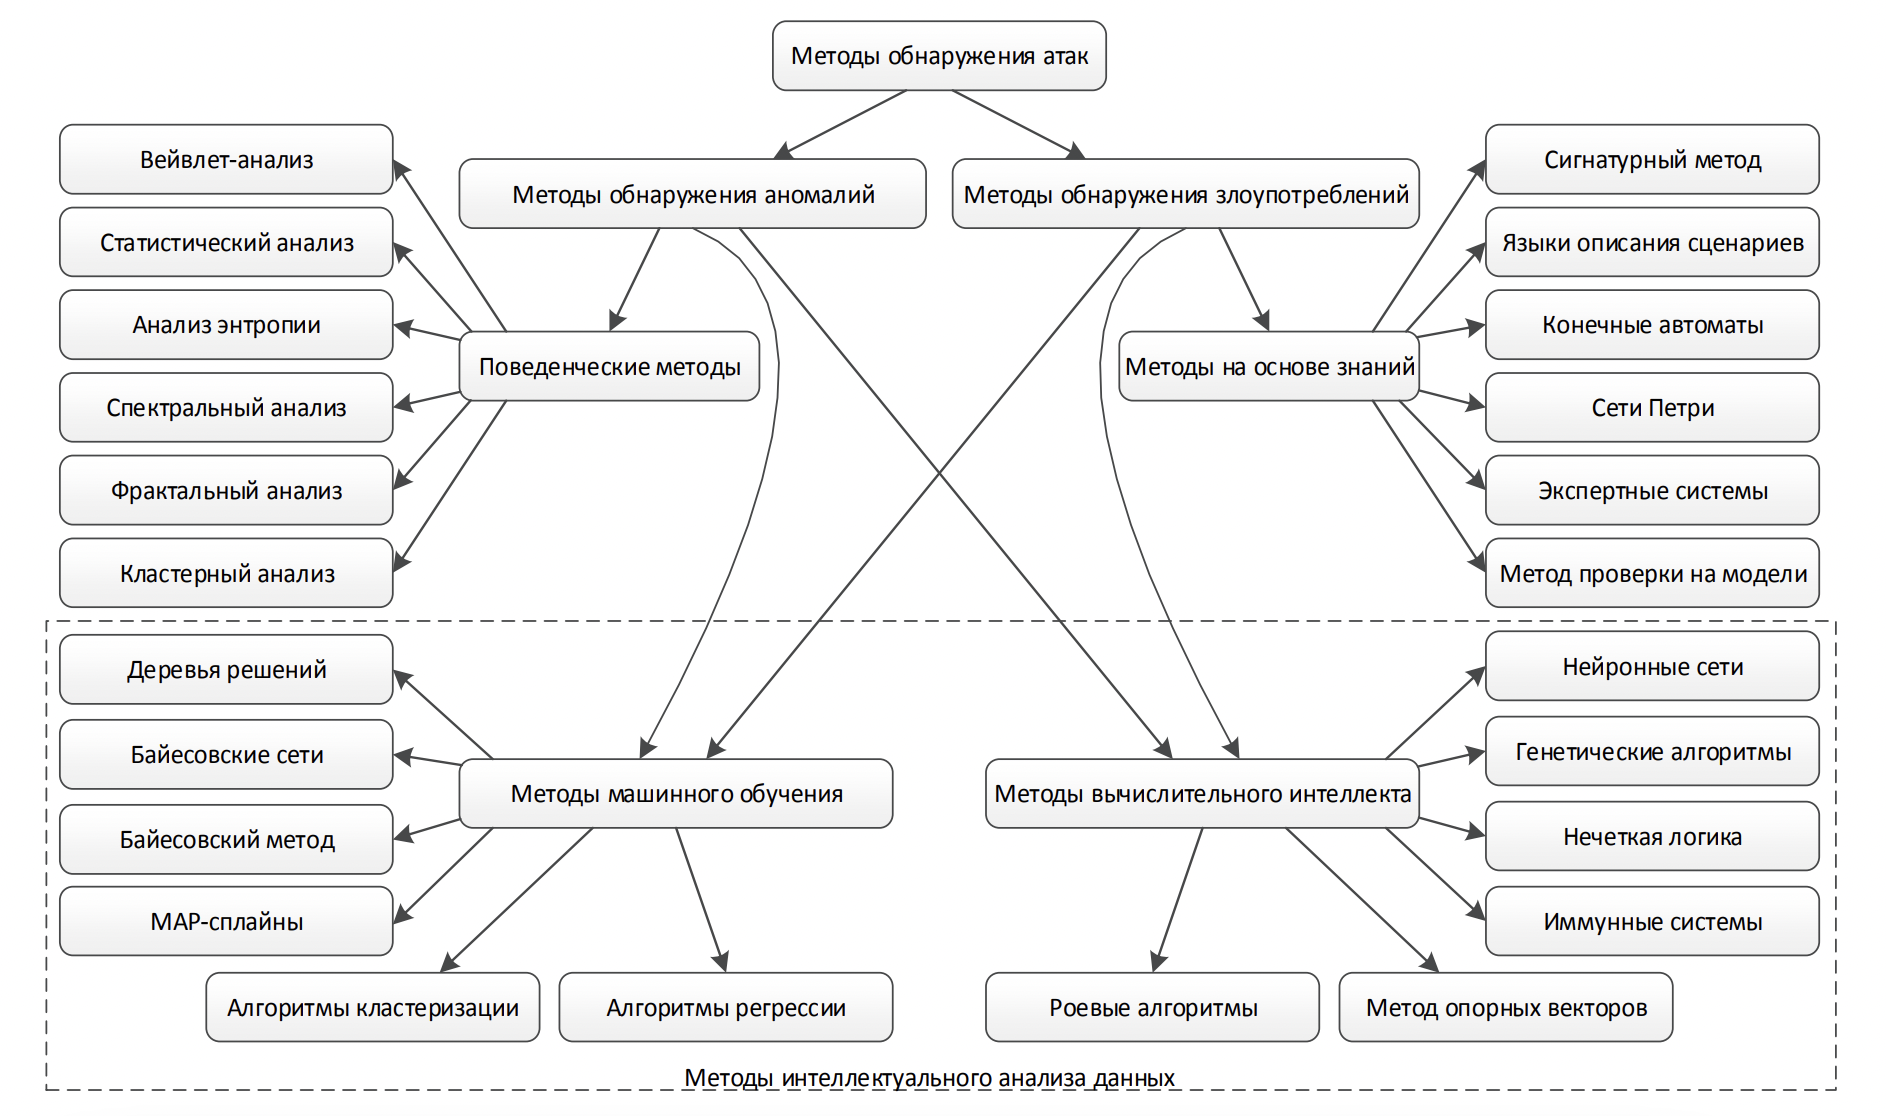
\includegraphics[width=1\textwidth]{inc/img/clasification.png}
%  \caption{Классификация методов обнаружения атак~\cite{браницкий2016анализ}}
%  \label{img:clasification}
% \end{figure}

\section*{Методы обнаружения SYN-flood атак}

Основной признак SYN-flood атак --- деградация онлайн-сервиса, а также полная или частичная недоступность IT-систем. Анализ трафика помогает обнаружить атаку и по косвенным признакам, таким как наличие повышенного количества SYN-запросов (SYN-запросы являются нормальной частью установки TCP-соединения, но их избыток может указывать на возможную атаку), подозрительные скачки объёмов трафика с одного IP-адреса (или диапазона IP-адресов). 

Кроме анализа трафика для обнаружения SYN-flood атак также используется анализ полуоткрытых соединений и задержек. Эксперименты показывают, что метод исследования задержек способен распознать те полуоткрытые соединения, которые вызваны SYN flood-атакой, и те, которые вызваны другими причинами. Метод получает задержки маршрутизаторов, посылая пакеты, содержащие специально установленные значения TTL в заголовке IP. Результаты зондирования используются затем для надёжного обнаружения SYN-флуда~\cite{корнев2012активные}.

% \begin{itemize}
%     \item[---] наличие повышенного количества SYN-запросов. SYN-запросы являются нормальной частью установки TCP-соединения, но их избыток может указывать на возможную атаку.;
%     \item[---] подозрительные скачки объёмов трафика с одного IP-адреса (или диапазона IP-адресов);
% \end{itemize}

% Общий алгоритм выявления сетевых атак может быть описан следующим образом. Данными для анализа является сетевой трафик, представленный как набор сетевых пакетов. Собранные сырые данные в дальнейшем послужат источником при формировании необходимой информации для последующего анализа. Так, полученные данные могут
% быть агрегированы за определенный временной интервал и нормализованы с целью задания признаковых атрибутов общего вида, которые
% потребуются при построении текущего профиля активности. Созданный набор признаков сравнивается с набором характеристик нормальной деятельности объекта (пользователя или системы) --- шаблоном
% нормального поведения. Существенное расхождение
% сравниваемых параметров фиксируется. Иначе происходит уточнение шаблона нормального поведения
% посредством изменения параметров его настройки с учетом текущего
% наблюдаемого профиля сетевой активности. 


% Для обнаружения аномалий используется общий подход выявления отличного от ожидаемого поведения. В рамках данного подхода выполняется накопление исторических данных о поведении некоторого параметра. 

% Для определения ожидаемого поведения анализируемого парамтра выполняется анализ исторических данных о поведении параметра. 

% Одним из возможных подходов к анализу исторических данных о поведении некоторого параметра --- нахождение среднего значения данного параметра за определенный, строго фиксированный, промежуток времени. Такой подход позволяет корректно обрабатываеть глобальные изменения в поведении анализируемого параметра, но допускает значительные неточности при прогнозировании поведения параметра.

% Другим возможным подходом к анализу исторических данных о поведении некоторого параметра --- является математическое апроксимация исторических данных о поведении некоторого параметра. Такой подход позволяет корректно обрабатываеть глобальные изменения в поведении анализируемого параметра, позволяет добиться высокого уровняточности при прогнозировании поведения анализируемого параметра, но имеет большую вычислительную сложность, чем нахождение среднего значения временного ряда.

% Таким образом для предсказания поведения анализируемого параметра решено использовать нахождение среднего значения временного ряда за фиксированный промежуток времени.

% Для определения области допустимых значений параметра используется некторый коэффициент, который в простейшем случае представлен фиксированным значением. Данный коэффициент представляет степень отклонения параметра от предсказанного значение. 

% В случае, если степень отклонения параметра превышает заданный коэффициент, рассматриваемое состояние параметра считается аномалией. Таким образом для отдельно взятого параметра можно выделить два типа аномалий: параметр больше ожидаемого значения, параметр меньше ожидаемого значения.

\section{Выбор отслеживаемых параметров сетевого трафика}

Анализируется заголовок сетевого и транспортного уровня, при обработке учитывается информация об IP-адресе отправителя, размере пакета, наличии выставленного флага SYN.
% Перехват пакетов происходит на сетевом уровне (уровнь 3 сетевой модели OSI), и при их обработке учитывается информация об IP-адресе отправителя, размере перехваченного пакета (в байтах).

% Отслеживаемые параметры представляют агрегированную информацию за фиксированный промежуток времени, которая регулярно сбрасывается.

В качестве отслеживаемых параметров выбраны: суммарное количество перехваченных TCP-пакетов, суммарное количество перехваченных TCP-пакетов с флагом SYN = 1, количество уникальных перехваченных IPv4 адресов, суммарный объем перехваченного трафика (в байтах), суммарное количество перехваченных пакетов, среднее значение суммарного объема перехваченного трафика с одного IPv4 адреса, максимальное значение суммарного объема перехваченного трафика с одного IPv4 адреса, среднее количество перехваченных пакетов с одного IPv4 адреса, максимальное количество перехваченных пакетов с одного IPv4 адреса.

% Отслеживание данных параметров позволяет выполнить базовый анализ входящего трафика на наличие аномалий.

Отслеживаемые параметры содержатся в заголовках IPv4 и TCP, по этой причине для получения отслеживаемых данных необходимо анализировать заголовоки IPv4 и TCP (сетевого и транспортного уровня).

\section{Программный интерфейс для сетевого взаимодействия в ОС Linux}
Программный интерфейс для сетевого взаимодействия в ОС Linux построен на стеке BSD. В этой подсистеме прием и передача данных на транспортном и сетевом уровнях модели OSI происходят с помощью интерфейса сокетов.

Когда в сетевую подсистему приходит пакет, возникает прерывание. Обработчик прерывания от сетевого адаптера копирует пакет в ядро, где тот ставится в так называемую буферную очередь и ожидает обработки соответствующим потоком ядра, и вызывает соответствующий softirq, который будет запущен демоном ksoftirqd и закончит обработку данного сетевого пакета (рисунок \ref{img:softirq})~\cite{ryaz}. 

\newpage
%\clearpage
\begin{figure}[h]
	\centering
	\begin{center}
		{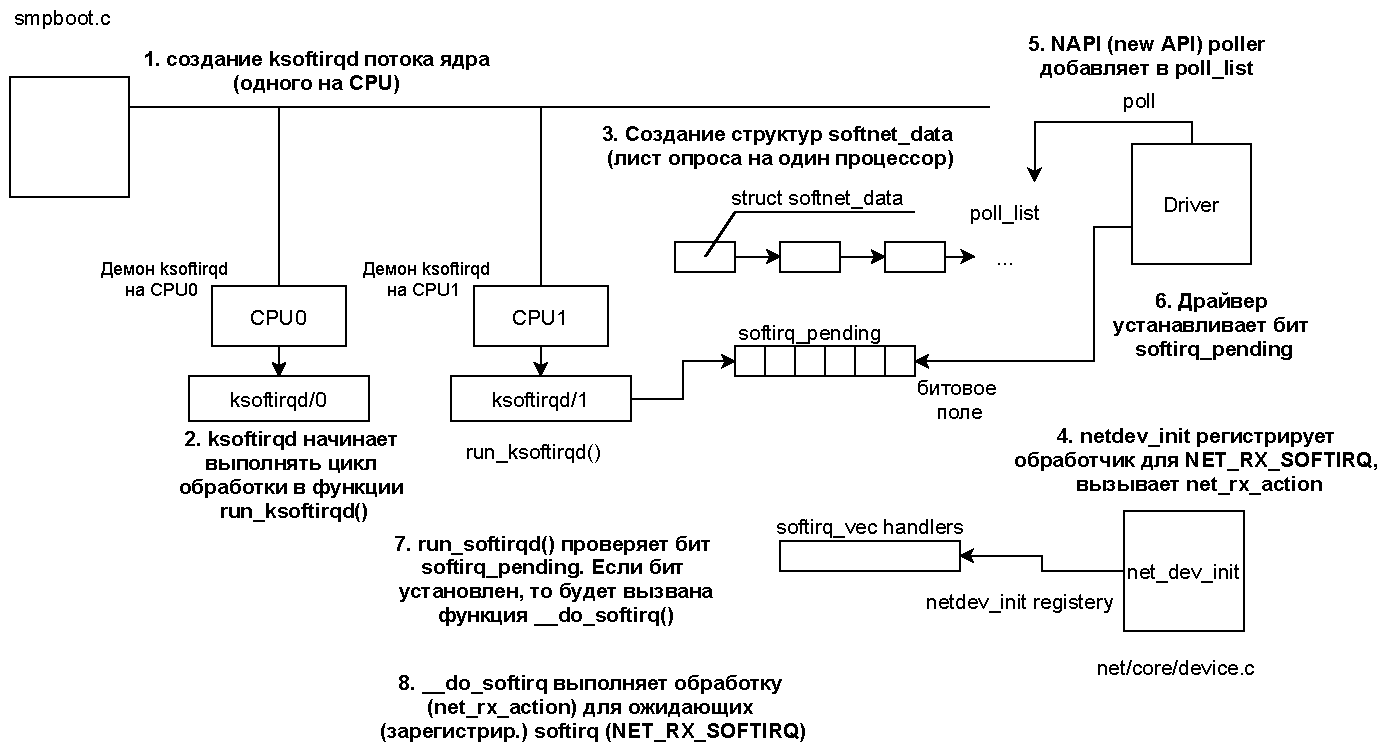
\includegraphics[scale=0.7]{inc/img/daemon.pdf}}
		\caption{Порядок выполняемых действий при приеме сетевого пакета}
		\label{img:softirq}
	\end{center}
\end{figure} 


Для обработки сетевых пакетов, поступающих с высокоскоростных интерфейсов, в Linux был добавлен NAPI (New API). В этом API механизм прерываний сочетается с механизмом опроса, и его основная цель -- сократить количество прерываний, генерируемых при получении пакета. В NAPI-совместимых драйверах при поступлении пакета прерывания отключаются, и обработчик только вызывает планировщик rx\_scheduler, который гарантирует, что в дальнейшем обработка пакета будет выполнена \cite{b5}.

На рассматриваемых уровнях модели OSI и происходит фильтрация пакетов с учетом информации о протоколе и об IP-адресах и номерах портов источника и назначения. Широко распространённым средством фильтрации сетевых пакетов является библиотека Netfilter.

\section{Фреймворк Netfilter}

Netfilter - это фреймворк, который предоставляется ядром ОС Linux, предоставляющая функционал для фильтрации и перенаправления пакетов~\cite{b7}. Netfilter представляет собой набор перехватчиков внутри ядра, позволяющий модулям ядра регистрировать функции обратного вызова в сетевом стеке. Эти функции вызываются для каждого пакета, который удовлетворяет соответствующему правилу перехвата~\cite{netfilter}.


Netfilter позволяет перехватить пакет в любой из пяти стандартных точек, через которые он проходит (рисунок \ref{img:packets}):


\begin{enumerate}
	\item NF\_INET\_PRE\_ROUTING -- все входящие пакеты;
	\item NF\_INET\_LOCAL\_IN -- входящие пакеты, предназначенные для локального процесса;
	\item NF\_INET\_FORWARD -- транзитные пакеты (предназначенные для другого интерфейса);
	\item NF\_INET\_LOCAL\_OUT -- исходящие пакеты, сформированные локальными процессами;
	\item NF\_INET\_POST\_ROUTING -- все исходящие пакеты (поступившие из точки NF\_INET\_FORWARD или сформированные локальными процессами).
\end{enumerate}

\begin{figure}[h]
	\centering
	\begin{center}
		{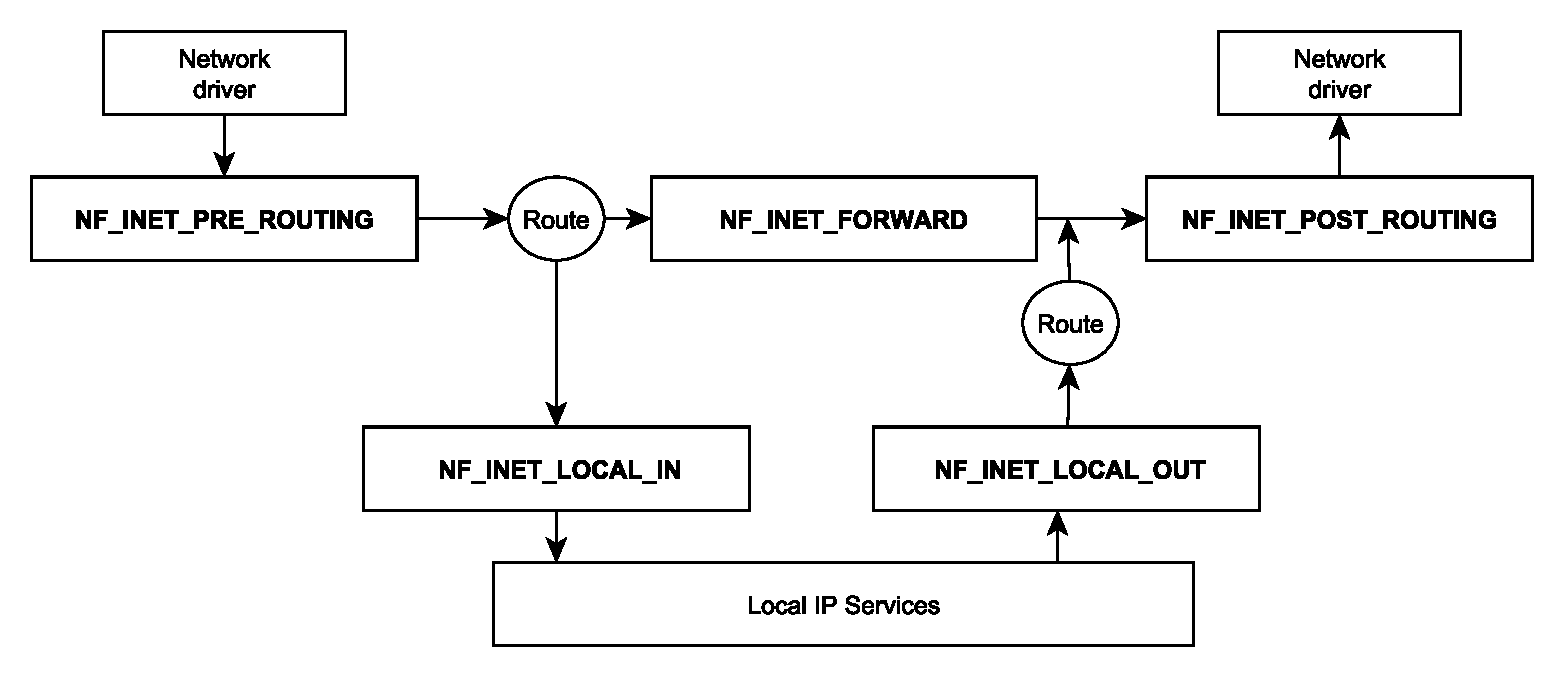
\includegraphics[scale=0.6]{inc/img/packets.pdf}}
		\caption{Точки, через которые проходит сетевой пакет}
		\label{img:packets}
	\end{center}
\end{figure} 

\section*{Функции перехвата}
Чтобы перехватить пакет в одной из перечисленных ранее точек, к ней необходимо подключить функцию перехвата (hook, ловушку). Для этого сначала необходимо заполнить структуру nf\_hook\_ops, основные поля которой приведены в листинге \ref{lst:hook}.

\begin{lstlisting}[caption = {Структура struct nf\_hook\_ops}, label=lst:hook]
struct nf_hook_ops {
	nf_hookfn		*hook;
	...
	u8			pf;
	...
	unsigned int		hooknum;
	int			priority;
};
\end{lstlisting}


Основные поля структуры:
\begin{itemize}
	\item[---] hook -- функция, которая будет вызвана для обработки пакета и принятия решения: отбросить или принять пакет;
	
	\item[---] pf -- семейство протоколов (PF\_INET для IPv4);
	
	\item[---] hooknum -- точка подключения функции;
	
	\item[---] priority -- приоритет (вводится, чтобы установить порядок вызова ловушек, подключенных к одной точке).
\end{itemize}

После заполнения структуры nf\_hook\_ops функцию перехвата необходимо зарегистрировать, вызвав функцию nf\_register\_net\_hook. Для удаления ловушки необходимо вызвать функцию nf\_unregister\_net\_hook. Прототипы этих функций приведены в листинге \ref{lst:hook_reg}.

\begin{lstlisting}[caption = {Функции для регистрации и удаления функций перехвата}, label=lst:hook_reg]
	int nf_register_net_hook(struct net *net, const struct nf_hook_ops *ops);

	void nf_unregister_net_hook(struct net *net, const struct nf_hook_ops *ops);
\end{lstlisting}

Прототип функции перехвата приведен в листинге \ref{lst:hook2}.

\begin{lstlisting}[caption = {Прототип функции-ловушки}, label=lst:hook2]
typedef unsigned int nf_hookfn(void *priv, struct sk_buff *skb, const struct nf_hook_state *state);
\end{lstlisting}

Аргументы функции:
\begin{itemize}
	\item[---] priv -- код одной из пяти точек подключения ловушки;
	\item[---] skb -- указатель на структуру sk\_buff, содержащую информацию о сетевом пакете; 
	\item[---] state -- указатель на структуру nf\_hook\_state, содержащую информацию, связанную с перехватом пакета (интерфейс ввода/вывода, приоритет и т.\,д.).
\end{itemize}

Все сетевые пакеты в ядре представляются структурой struct sk\_buff, поля которой приведены в листинге \ref{lst:sk_buff}.


\begin{lstlisting}[caption = {Структура struct sk\_buff}, label=lst:sk_buff]
	struct sk_buff {
		/* временная метка */
		ktime_t     tstamp;
		
		/* указатель на сокет, который отправил или получил этот пакет */
		struct sock     *sk;
		
		/* указатель на устройство, с которого получен или которому будет отправлен пакет */
		struct net_device   *dev;
		
		/* L3 протокол */
		__be16          protocol;
		
		/* смещения заголовков относительно head */
		__u16           transport_header;
		__u16           network_header;
		__u16           mac_header;
		
		/* указатели на конец и начало данных */
		sk_buff_data_t      tail;
		sk_buff_data_t      end;
		
		/* 
		head - указатель на начало буфера выделенного под данные
		data - указатель на начало данных. 
		*/
		unsigned char       *head, *data;
		
		// счетчик ссылок 
		atomic_t        users;
	};
\end{lstlisting}

\section{Анализ способа изменения видимости модуля}
Для того, чтобы заинтересованный пользователь не смог удалить средство контроля трафика, его необходимо сделать невидимым. Удаляя соответствующий элемент из связного списка модулей, он становится скрытым, и система не может предоставить информацию о данном загружаемом модуле.

Для взаимодействия со списком модулей необходимо использовать структуру \textbf{struct list\_head} и функции \textbf{list\_add}, \textbf{list\_del}. Перед удалением модуля из списка, следует сохранить его указатель для обеспечения возможности восстановить его видимость.

Структура \textbf{struct module} (Листинг \ref{lst:struct_module}), описывающая модуль, предоставляет доступ к связному списку, где поле list -- его элемент.
\begin{lstlisting}[caption = {struct module}, label=lst:struct_module]
struct module
{
	enum module_state state;
	struct list_head list; /* Member of list of modules */
	char name[MODULE_NAME_LEN]; /* Unique handle for this module */
	...
};
\end{lstlisting}

% \newpage


\section{Требования к программному обеспечения для взаимодействия с загружаемым модулем ядра для ОС Linux}

ПО для взаимодействия с разрабатываемым загружаемым модулем ядра для ОС Linux создается для исключения возможности попадания некорректных данных в пространство ядра и облегчения взаимодействия пользователя с загружаемым модулем ядра.

Задача данного ПО --- передать данные полученные от пользователя, в фиксированном формате, в пространство ядра.

Для взаимодействия с загружаемым модулем ядра для ОС Linux через стороннее ПО необходимо реализовать возможность:

\begin{itemize}
    \item[---] демонстрировать статус работы загружаемого модуля ядра для ОС Linux;
    \item[---] демонстрировать анализируемые модулем параметры трафика;
    \item[---] скрывать загружаемым модуль ядра для ОС Linux;
    \item[---] восстанавливать видимость загружаемого модуля ядра для ОС Linux;
\end{itemize}

Далее рассмотрены разработанные для описанного ПО типы данных.

В листинге \ref{lst:command_type} приведен тип данных, который описывает выполняемое пользователем действие.
\begin{lstlisting}[caption = {command\_type}, label=lst:command_type]
enum command_type {
    UNDEFINED = 0,
    HIDE = 1,
    UNHIDE = 2,
};
\end{lstlisting}

В листинге \ref{lst:command} приведен тип данных, который описывает информацию, которая передается в пространство ядра.
\begin{lstlisting}[caption = {command}, label=lst:command]
struct command
{
    enum command_type type;
};
\end{lstlisting}

В листинге \ref{lst:l2_property} приведен тип данных, который описывает отслеживаемый параметр.
\begin{lstlisting}[caption = {l2\_property}, label=lst:l2_property]
enum l2_property {
    L2_PROPERTY_UNDEFINED = 0,
    L2_PROPERTY_UNIQUE_SADDRS_COUNT = 1,
    L2_PROPERTY_CATCHED_PACKETS_COUNT = 2,
    L2_PROPERTY_TOT_LEN = 3,
    L2_PROPERTY_AVG_CATCHED_PACKETS = 4,
    L2_PROPERTY_MAX_CATCHED_PACKETS = 5,
    L2_PROPERTY_AVG_LEN = 6,
    L2_PROPERTY_MAX_LEN = 7,
    L2_PROPERTY_TOT_TCP = 8,
    L2_PROPERTY_TOT_SYN = 9,
};
\end{lstlisting}

% В листинге \ref{lst:l2_anomaly_type} приведен тип данных, который описывает тип выявленной аномалии.
% \begin{lstlisting}[caption = {l2\_anomaly\_type}, label=lst:l2_anomaly_type]
% enum l2_anomaly_type {
%     L2_ANOMALY_TYPE_UNDEFINED = 0,
%     L2_ANOMALY_TYPE_INCREASE = 1,
%     L2_ANOMALY_TYPE_FALL = 2,
% };
% \end{lstlisting}

В листинге \ref{lst:l2_data_slice} приведен тип данных, который описывает отслеживаемые параметры трафика.
\begin{lstlisting}[caption = {l2\_data\_slice}, label=lst:l2_data_slice]
struct l2_data_slice
{
    uint64_t from_time;
    uint32_t unique_saddr_count;
    uint32_t catched_packets_count;
    uint32_t tot_len;
    uint32_t avg_catched_packets;
    uint32_t max_catched_packets;
    uint32_t avg_len;
    uint32_t max_len;
    int crit_behaviour;
    enum l2_property property;
    enum l2_crit_behaviour_type type;
    uint32_t tot_tcp;
    uint32_t tot_syn;
};
\end{lstlisting}

В листинге \ref{lst:module_stats} приведен тип данных, который описывает статус работы загружаемого модуля ядра для ОС Linux.
\begin{lstlisting}[caption = {module\_stats}, label=lst:module_stats]
struct module_stats
{
    uint32_t history_length;
    uint32_t current_history_length;
    uint64_t current_periud_ns;
    uint32_t crit_behaviour_count;
    uint64_t first_crit_behaviour_ns;
    uint64_t last_crit_behaviour_ns;
};
\end{lstlisting}

% \section{Анализ методов динамического обнаружения аномалий}
% Для обнаружения аномалий используется общий подход выявления отличного от ожидаемого поведения. В рамках данного подхода выполняется накопление исторических данных о поведении некоторого параметра. 

% Для определения ожидаемого поведения анализируемого парамтра выполняется анализ исторических данных о поведении параметра. 

% Одним из возможных подходов к анализу исторических данных о поведении некоторого параметра --- нахождение среднего значения данного параметра за определенный, строго фиксированный, промежуток времени. Такой подход позволяет корректно обрабатываеть глобальные изменения в поведении анализируемого параметра, но допускает значительные неточности при прогнозировании поведения параметра.

% Другим возможным подходом к анализу исторических данных о поведении некоторого параметра --- является математическое апроксимация исторических данных о поведении некоторого параметра. Такой подход позволяет корректно обрабатываеть глобальные изменения в поведении анализируемого параметра, позволяет добиться высокого уровняточности при прогнозировании поведения анализируемого параметра, но имеет большую вычислительную сложность, чем нахождение среднего значения временного ряда.

% Таким образом для предсказания поведения анализируемого параметра решено использовать нахождение среднего значения временного ряда за фиксированный промежуток времени.

% Для определения области допустимых значений параметра используется некторый коэффициент, который в простейшем случае представлен фиксированным значением. Данный коэффициент представляет степень отклонения параметра от предсказанного значение. 

% В случае, если степень отклонения параметра превышает заданный коэффициент, рассматриваемое состояние параметра считается аномалией. Таким образом для отдельно взятого параметра можно выделить два типа аномалий: параметр больше ожидаемого значения, параметр меньше ожидаемого значения.

\section{Выводы}

В результате проведенного анализа был выбран способ перехвата входящих пакетов --- путем регистрации функций перехвата с использованием фреймворка Netfilter. В качестве точки перехвата предлагается использовать точку, в которую проходят пакеты адресованные локальному процессу (NF\_INET\_LOCAL\_IN).

Были рассмотрены структуры и функции ядра, предоставляющие  информацию о сетевых пакетах, был рассмотрен метод сокрытия загружаемого модуля ядра ОС Linux.

Отслеживаемые параметры представляют агрегированную информацию за фиксированный промежуток времени, которая регулярно сбрасывается.

В качестве отслеживаемых параметров выбраны: суммарное количество перехваченных TCP-пакетов, суммарное количество перехваченных TCP-пакетов с флагом SYN = 1, количество уникальных перехваченных IPv4 адресов, суммарный объем перехваченного трафика (в байтах), суммарное количество перехваченных пакетов, среднее значение суммарного объема перехваченного трафика с одного IPv4 адреса, максимальное значение суммарного объема перехваченного трафика с одного IPv4 адреса, среднее количество перехваченных пакетов с одного IPv4 адреса, максимальное количество перехваченных пакетов с одного IPv4 адреса.

Для анализа исторических данных использовался поиск средних значений анализируемых параметров~\cite{карачанская2019метод}. Такой подход позволяет корректно обрабатываеть глобальные изменения в поведении анализируемого параметров.

% ***************************************************************************

\chapter{Конструкторский раздел}

\section{IDEF0}

На рисунках \ref{img:IDEF00}-\ref{img:IDEF01} представлена IDEF0-диаграмма, описывающая работу разрабатываемого программного обеспечения.

\begin{figure}[hbtp]
 \centering
 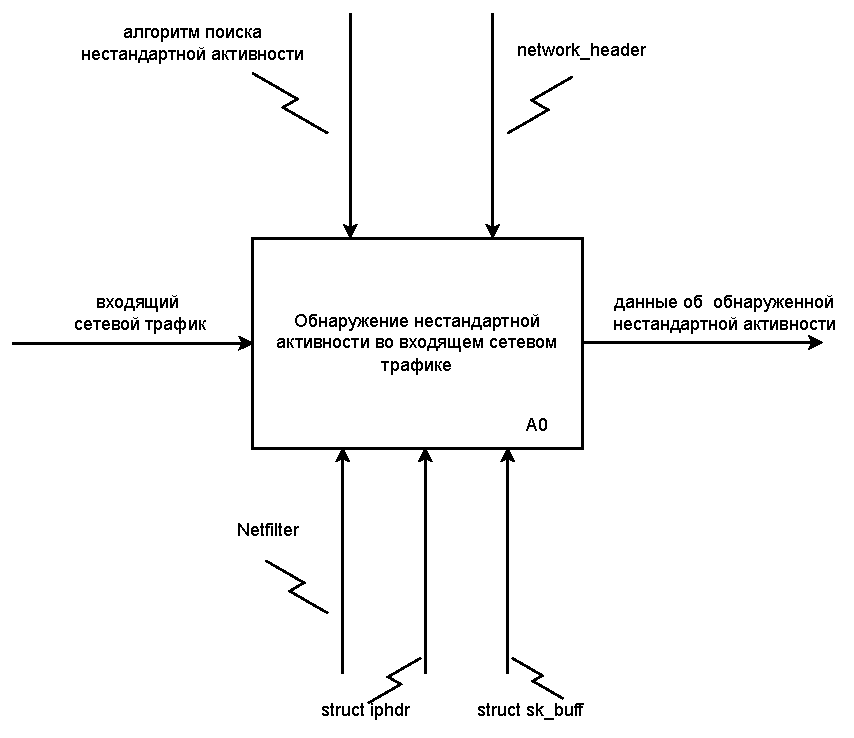
\includegraphics[width=0.7\textwidth]{inc/img/idfe00.pdf}
 \caption{Отслеживание сетевого трафика, верхний уровень}
 \label{img:IDEF00}
\end{figure}

% \clearpage
\begin{figure}[hbtp]
 \centering
 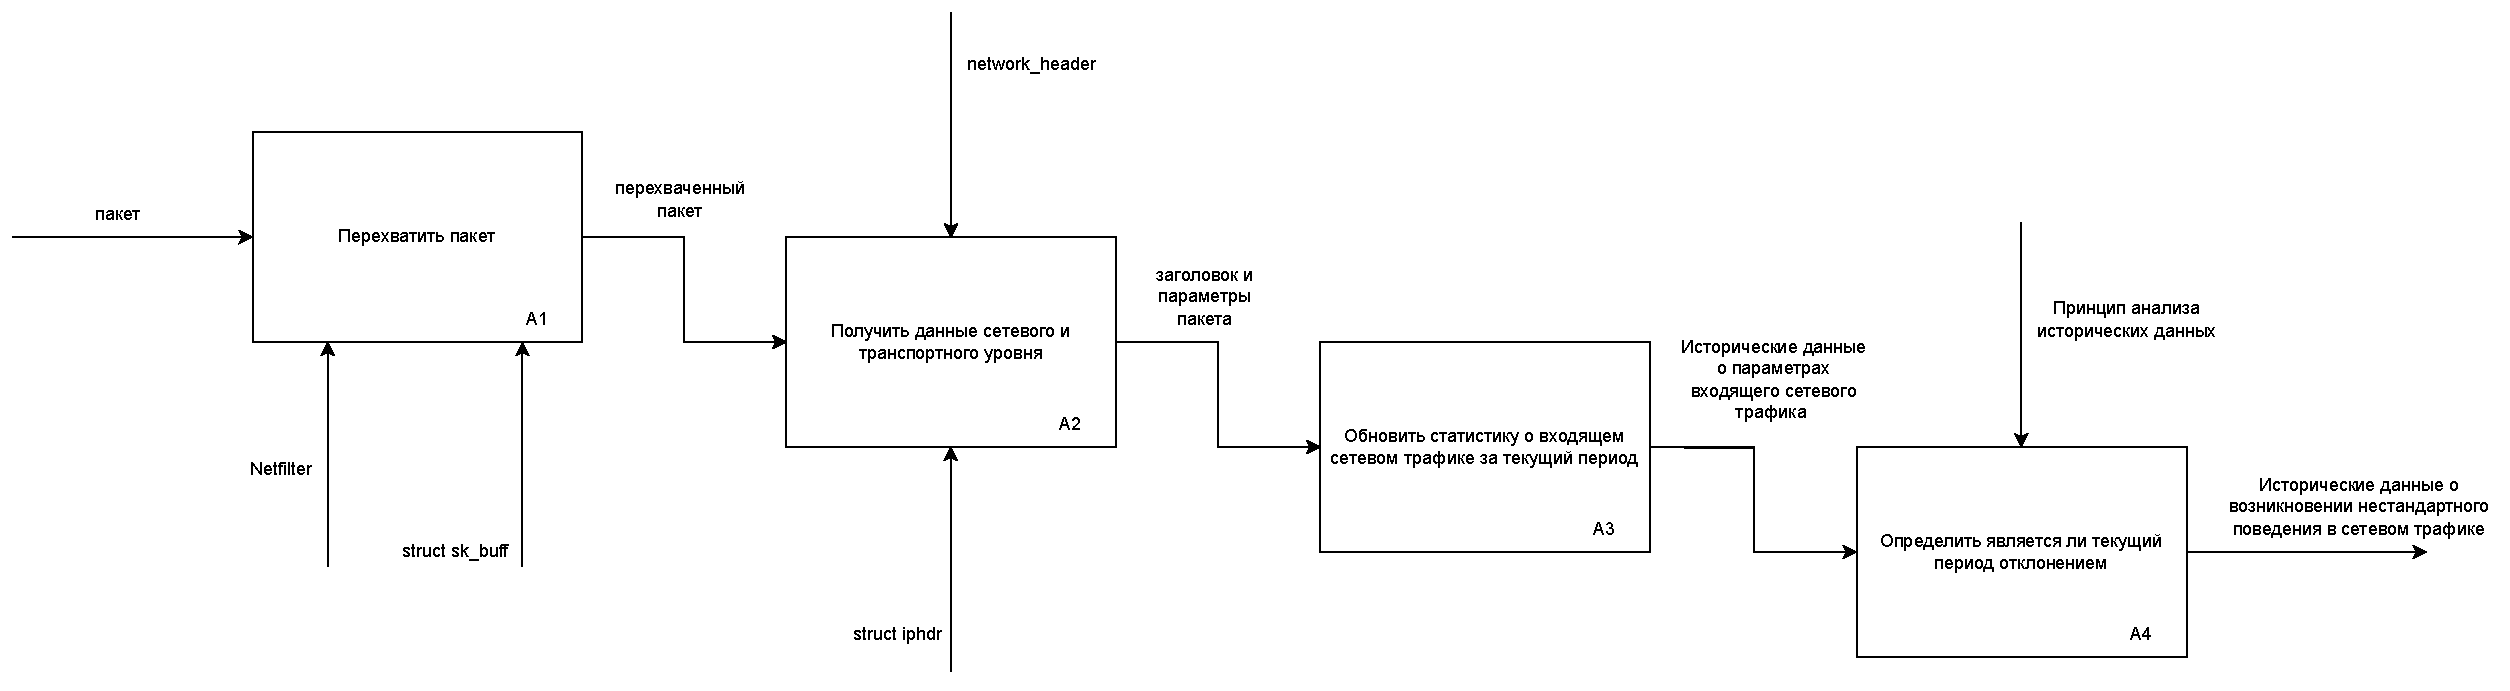
\includegraphics[width=0.99\textwidth]{inc/img/idfe01.pdf}
 \caption{Отслеживание сетевого трафика, нижний уровень}
 \label{img:IDEF01}
\end{figure}

\newpage
\section{Структура программного обеспечения}
Разрабатываемое ПО должено быть реализован в виде загружаемого модуля ядра и работать в режиме ядра. Однако пользователь должен иметь возможность управлять работой ПО (скрывать модуль и восстанавливать его видимость), для чего необходимо разработать отдельное приложение, которое будет выполняется в режиме пользователя.

Структура программного обеспечения приведена на рисунке \ref{img:structure}.

\begin{figure}[hbtp]
 \centering
 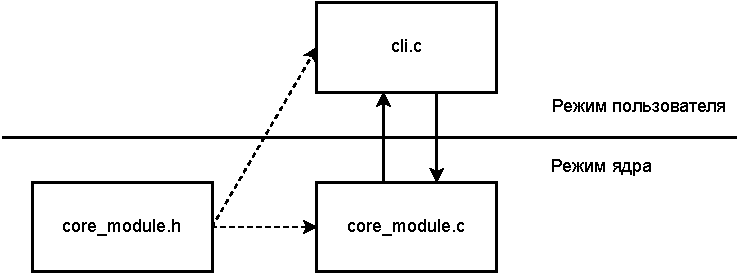
\includegraphics[width=0.7\textwidth]{inc/img/po_struct.pdf}
 \caption{Структура программного обеспечения}
 \label{img:structure}
\end{figure}

\newpage
\section{Алгоритм инициализации модуля}
На рисунке \ref{img:register} приведен алгоритм инициализации модуля.

\begin{figure}[hbtp]
 \centering
 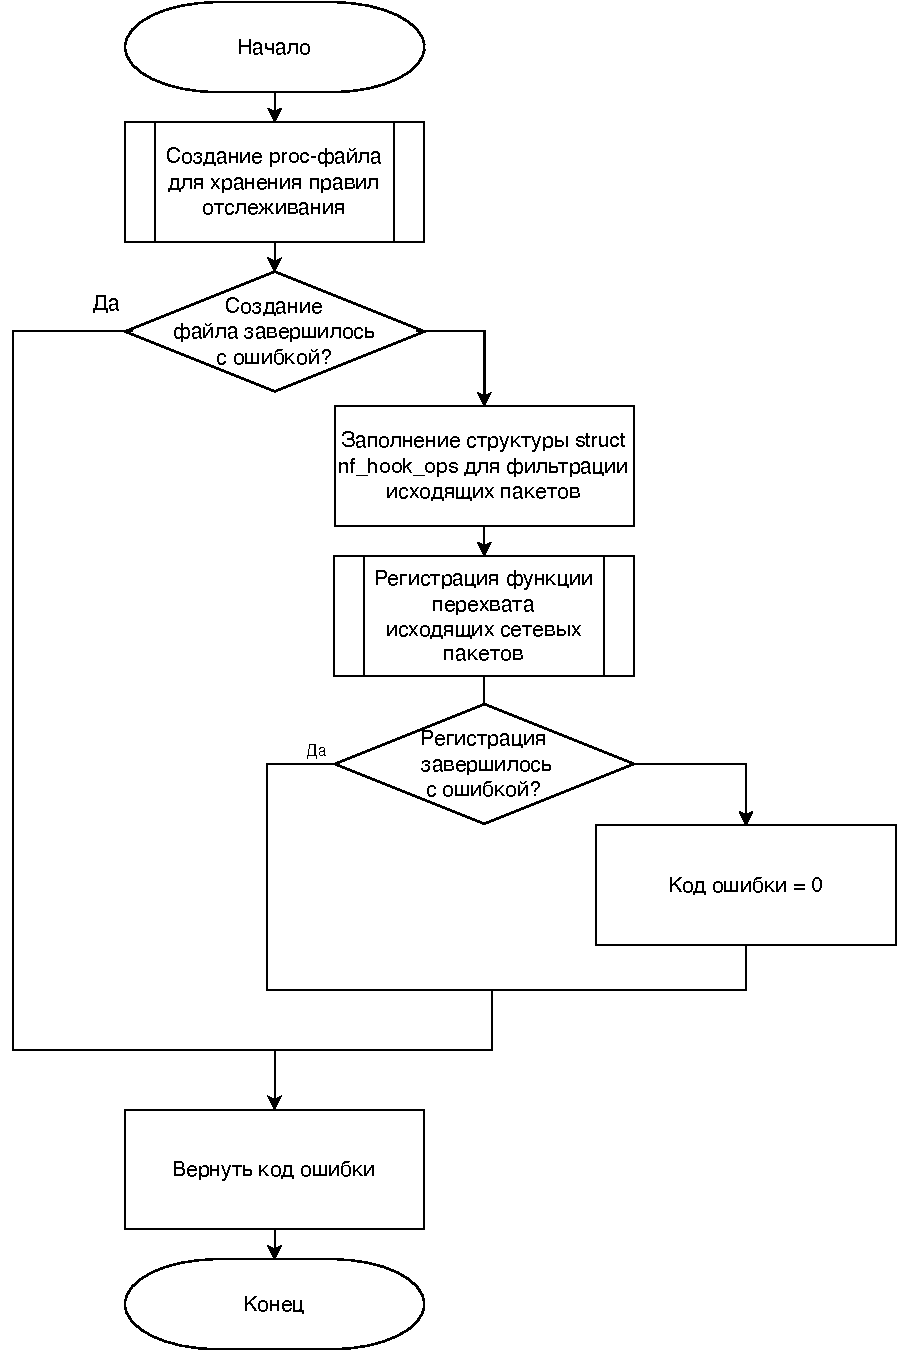
\includegraphics[width=0.7\textwidth]{inc/img/init.pdf}
 \caption{Алгоритм инициализации модуля}
 \label{img:register}
\end{figure}

\newpage
\section{Алгоритм обработки перехваченного сетевого пакета}
На рисунке \ref{img:filter} приведен алгоритм обработки перехваченного сетевого пакета.

\begin{figure}[hbtp]
 \centering
 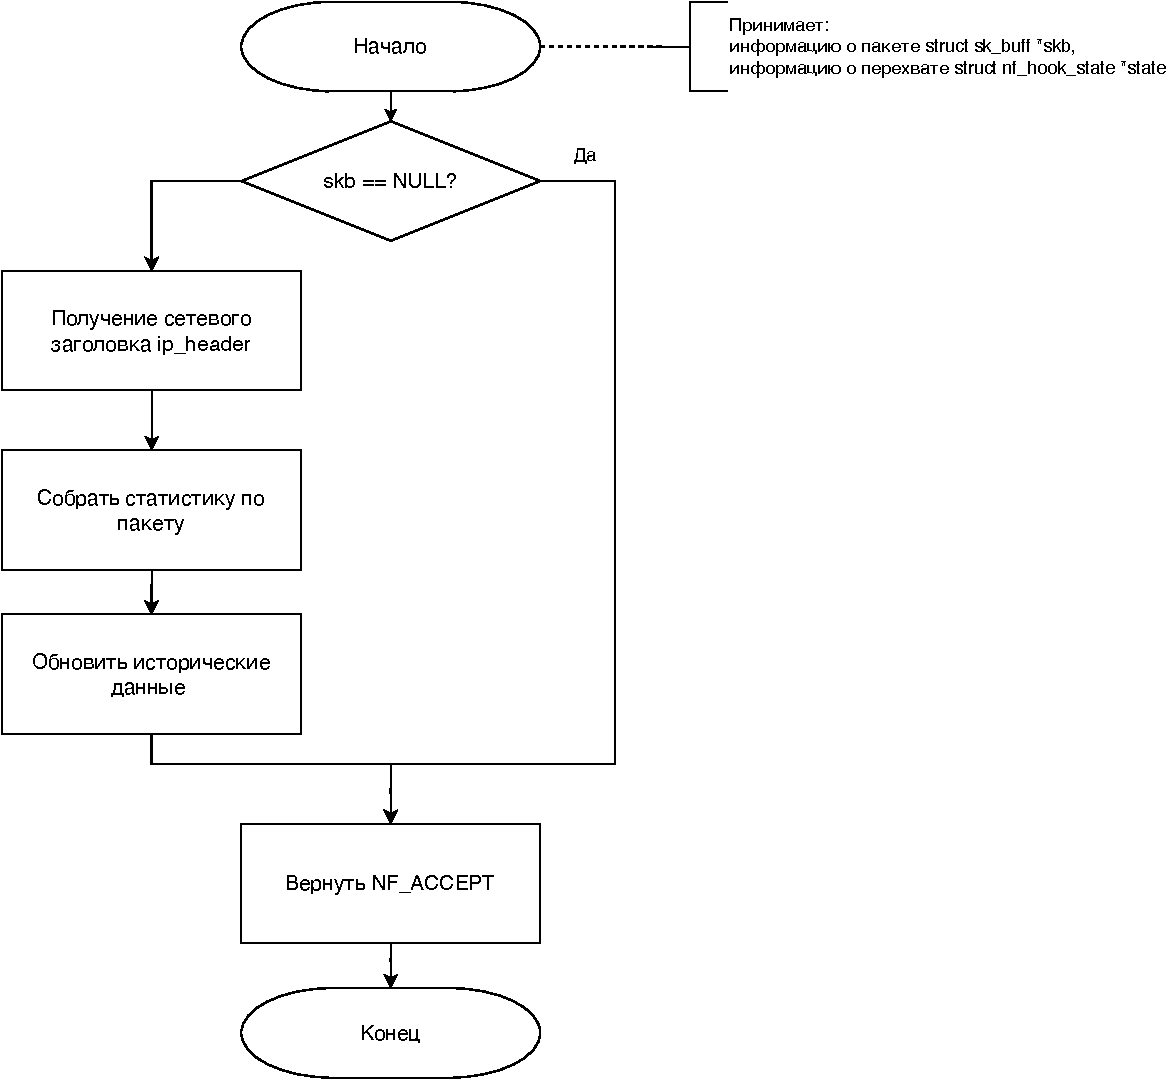
\includegraphics[width=0.9\textwidth]{inc/img/catch.pdf}
 \caption{Алгоритм обработки перехваченного сетевого пакета}
 \label{img:filter}
\end{figure}

\newpage
\section{Алгоритм обнаружение атак в исторических данных}
На рисунке \ref{img:anomaly} приведен алгоритм обнаружение аномалий в исторических данных для определенного параметра.

\begin{figure}[hbtp]
 \centering
 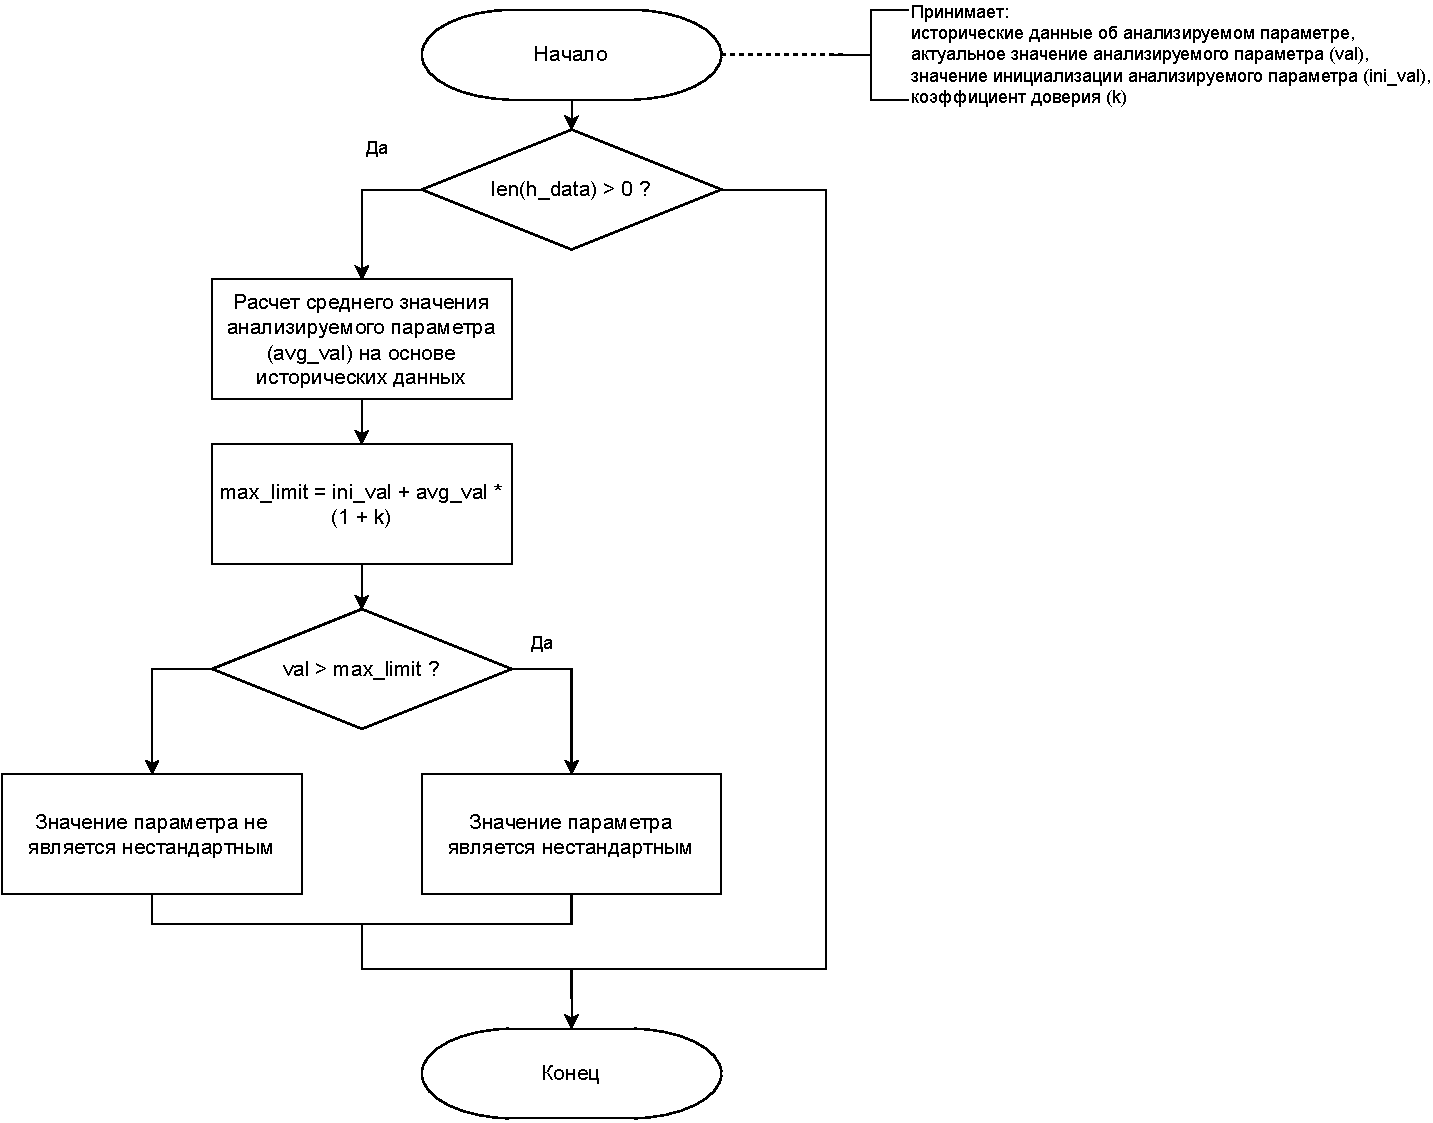
\includegraphics[width=0.9\textwidth]{inc/img/increase.pdf}
 \caption{Алгоритм обнаружения атак в исторических данных}
 \label{img:anomaly}
\end{figure}

% ***************************************************************************

\chapter{Технологический раздел}

\section{Выбор средств разработки}
В качестве языка программирования для реализации поставленной задачи был выбран язык Си. Для сборки модуля использовалась утилита make. В качестве среды разработки был выбран Qt Creator\cite{qt}, так как он кроссплатформенный, бесплатный и использовался в курсе программирования ранее. 

\section{Сборка и запуск модуля}
Сборка модуля осуществляется командой make. На листинге \ref{lst:make} приведено содержимое Makefile.

\begin{lstlisting}[caption = {Makefile}, label=lst:make]
obj-m += core_module.o

all: interface.o core_module.o

interface.o: interface.c module.h
	gcc -o interface.o interface.c	

core_module.o: core_module.c
	make -C /lib/modules/$(shell uname -r)/build M=$(PWD) modules

clean:
	rm -rf fw *.o
	make -C /lib/modules/$(shell uname -r)/build M=$(PWD) clean
\end{lstlisting}

Для того, чтобы загрузить модуль, нужно воспользоваться командой \textbf{sudo insmod core\_module.ko}, для того, чтобы выгрузить -- \textbf{sudo rmmod core\_module}.

\section{Инициализация модуля}
В листинге~\ref{lst:init} приведена реализация функции инициализации модуля.

\begin{lstlisting}[caption = {Функция инициализации модуля}, label=lst:init]
static int __init my_module_init(void) {
    int rc = 0;

    nf_register_net_hook(&init_net, &module_hook_ops);

    rc = misc_register(&dev_l2_data);
    if (rc)
    {
        printk(MODULE_DMESG_PREFIX "[ERROR] registration was failed");
        return rc;
    }

    rc = misc_register(&dev_stats);
    if (rc)
    {
        printk(MODULE_DMESG_PREFIX "[ERROR] registration was failed");
        return rc;
    }

    rc = misc_register(&dev_ctrl);
    if (rc)
    {
        printk(MODULE_DMESG_PREFIX "[ERROR] registration was failed");
        return rc;
    }

    printk(MODULE_DMESG_PREFIX "module was loaded");

    return 0;
}
\end{lstlisting}

\section{Обработка перехваченных сетевых пакетов}
В листинге~\ref{lst:in} приведена реализация функции обработки перехваченных сетевых пакетов.

\begin{lstlisting}[caption = {Функции обработки перехваченных сетевых пакетов}, label=lst:in]
static unsigned int catch_traffic(void *priv, struct sk_buff *skb, const struct nf_hook_state *state)
{
    struct iphdr *iph;  /* An IPv4 packet header */
    uint32_t saddr;
    uint32_t tot_len;

    if (!skb) return NF_ACCEPT;

    iph = (struct iphdr *)skb_network_header(skb);
    if (iph == NULL) return NF_ACCEPT;

    saddr = iph->saddr;
    tot_len = iph->tot_len;

    add_packet_info(saddr, tot_len);

    return NF_ACCEPT;
}
\end{lstlisting}

\section{Обнаружение признаков атак}
В листинге~\ref{lst:anomaly} приведена реализация функции обнаружения нестандартной активности во входящем сетевом трафике.

\begin{lstlisting}[caption = {Функции обнаружения нестандартного активности во входящем сетевом трафике}, label=lst:anomaly]
void inspect_last(void) {
    if (second_layer_table_next_index < 2) {
        return;
    }

    struct second_layer_schema avg_values = {
        .unique_saddr_count = 0,
        .catched_packets_count = 0,
        .tot_len = 0,
        .avg_catched_packets = 0,
        .max_catched_packets = 0,
        .avg_len = 0,
        .max_len = 0,
        .tot_tcp = 0,
        .tot_syn = 0,
    };

    for (int i = 0; i < second_layer_table_next_index - 1; i++) {
        avg_values.unique_saddr_count += second_layer_table[i].unique_saddr_count;
        avg_values.catched_packets_count += second_layer_table[i].catched_packets_count;
        avg_values.tot_len += second_layer_table[i].tot_len;
        avg_values.avg_catched_packets += second_layer_table[i].avg_catched_packets;
        avg_values.max_catched_packets += second_layer_table[i].max_catched_packets;
        avg_values.avg_len += second_layer_table[i].avg_len;
        avg_values.max_len += second_layer_table[i].max_len;
        avg_values.tot_tcp += second_layer_table[i].tot_tcp;
        avg_values.tot_syn += second_layer_table[i].tot_syn;
    }

    avg_values.unique_saddr_count /= (second_layer_table_next_index - 1);
    avg_values.catched_packets_count /= (second_layer_table_next_index - 1);
    avg_values.tot_len /= (second_layer_table_next_index - 1);
    avg_values.avg_catched_packets /= (second_layer_table_next_index - 1);
    avg_values.max_catched_packets /= (second_layer_table_next_index - 1);
    avg_values.avg_len /= (second_layer_table_next_index - 1);
    avg_values.max_len /= (second_layer_table_next_index - 1);
    avg_values.tot_tcp /= (second_layer_table_next_index - 1);
    avg_values.tot_syn /= (second_layer_table_next_index - 1);

    struct second_layer_schema last = second_layer_table[second_layer_table_next_index - 1];

    uint64_t limit;

    limit = avg_values.unique_saddr_count * (100 + eps_percent) / 100 + initial_vec.unique_saddr_count;
    if (last.unique_saddr_count > limit) {
        second_layer_table[second_layer_table_next_index - 1].crit_behaviour = 1;
        second_layer_table[second_layer_table_next_index - 1].property = CRIT_BEHAVIOUR_PROPERTY_UNIQUE_SADDRS_COUNT;
        second_layer_table[second_layer_table_next_index - 1].type = CRIT_BEHAVIOUR_TYPE_INCREASE;
        return;
    }

    limit = avg_values.catched_packets_count * (100 + eps_percent) / 100 + initial_vec.catched_packets_count;
    if (last.catched_packets_count > limit) {
        second_layer_table[second_layer_table_next_index - 1].crit_behaviour = 1;
        second_layer_table[second_layer_table_next_index - 1].property = CRIT_BEHAVIOUR_PROPERTY_CATCHED_PACKETS_COUNT;
        second_layer_table[second_layer_table_next_index - 1].type = CRIT_BEHAVIOUR_TYPE_INCREASE;
        return;
    }

    limit = avg_values.tot_len * (100 + eps_percent) / 100 + initial_vec.tot_len;
    if (last.tot_len > limit) {
        second_layer_table[second_layer_table_next_index - 1].crit_behaviour = 1;
        second_layer_table[second_layer_table_next_index - 1].property = CRIT_BEHAVIOUR_PROPERTY_TOT_LEN;
        second_layer_table[second_layer_table_next_index - 1].type = CRIT_BEHAVIOUR_TYPE_INCREASE;
        return;
    }

    limit = avg_values.avg_catched_packets * (100 + eps_percent) / 100 + initial_vec.avg_catched_packets;
    if (last.avg_catched_packets > limit) {
        second_layer_table[second_layer_table_next_index - 1].crit_behaviour = 1;
        second_layer_table[second_layer_table_next_index - 1].property = CRIT_BEHAVIOUR_PROPERTY_AVG_CATCHED_PACKETS;
        second_layer_table[second_layer_table_next_index - 1].type = CRIT_BEHAVIOUR_TYPE_INCREASE;
        return;
    }

    limit = avg_values.max_catched_packets * (100 + eps_percent) / 100 + initial_vec.max_catched_packets;
    if (last.max_catched_packets > limit) {
        second_layer_table[second_layer_table_next_index - 1].crit_behaviour = 1;
        second_layer_table[second_layer_table_next_index - 1].property = CRIT_BEHAVIOUR_PROPERTY_MAX_CATCHED_PACKETS;
        second_layer_table[second_layer_table_next_index - 1].type = CRIT_BEHAVIOUR_TYPE_INCREASE;
        return;
    }

    limit = avg_values.avg_len * (100 + eps_percent) / 100 + initial_vec.avg_len;
    if (last.avg_len > limit) {
        second_layer_table[second_layer_table_next_index - 1].crit_behaviour = 1;
        second_layer_table[second_layer_table_next_index - 1].property = CRIT_BEHAVIOUR_PROPERTY_AVG_LEN;
        second_layer_table[second_layer_table_next_index - 1].type = CRIT_BEHAVIOUR_TYPE_INCREASE;
        return;
    }

    limit = avg_values.max_len * (100 + eps_percent) / 100 + initial_vec.max_len;
    if (last.max_len > limit) {
        second_layer_table[second_layer_table_next_index - 1].crit_behaviour = 1;
        second_layer_table[second_layer_table_next_index - 1].property = CRIT_BEHAVIOUR_PROPERTY_MAX_LEN;
        second_layer_table[second_layer_table_next_index - 1].type = CRIT_BEHAVIOUR_TYPE_INCREASE;
        return;
    }

    limit = avg_values.tot_tcp * (100 + eps_percent) / 100 + initial_vec.tot_tcp;
    if (last.tot_tcp > limit) {
        second_layer_table[second_layer_table_next_index - 1].crit_behaviour = 1;
        second_layer_table[second_layer_table_next_index - 1].property = CRIT_BEHAVIOUR_PROPERTY_TOT_TCP;
        second_layer_table[second_layer_table_next_index - 1].type = CRIT_BEHAVIOUR_TYPE_INCREASE;
        return;
    }

    limit = avg_values.tot_syn * (100 + eps_percent) / 100 + initial_vec.tot_syn;
    if (last.tot_syn > limit) {
        second_layer_table[second_layer_table_next_index - 1].crit_behaviour = 1;
        second_layer_table[second_layer_table_next_index - 1].property = CRIT_BEHAVIOUR_PROPERTY_TOT_SYN;
        second_layer_table[second_layer_table_next_index - 1].type = CRIT_BEHAVIOUR_TYPE_INCREASE;
        return;
    }
}
\end{lstlisting}

\section{Изменение видимости модуля}
В листинге~\ref{lst:hide} приведена реализация функции сокрытия разработанного загружаемого модуля ядра ОС Linux.

\begin{lstlisting}[caption = {Функция сокрытия загружаемого модуля ядра}, label=lst:hide]
void hide(void)
{
    if (flag_hidden)
        return;

    module_prev = THIS_MODULE->list.prev;
    list_del(&THIS_MODULE->list);
    flag_hidden = 1;

    printk(">>> FIREWALL: module was hidden");
}
\end{lstlisting}

В листинге~\ref{lst:unhide} приведена реализация функции возобновления видимости разработанного загружаемого модуля ядра ОС Linux.

\begin{lstlisting}[caption = {Функция возобновления видимости загружаемого модуля ядра}, label=lst:unhide]
void unhide(void)
{
    if (!flag_hidden)
        return;
    list_add(&THIS_MODULE->list, module_prev);
    flag_hidden = 0;
    printk(">>> FIREWALL: module was exposed");
} 
\end{lstlisting}

% ***************************************************************************

\chapter{Исследовательский раздел}

\section{Команды}
Для того, чтобы посмотреть все команды и формат задаваемых правил, необходимо вызвать \textbf{help}. На Рисунке \ref{img:help} представлен результат.

\begin{figure}[hbtp]
 \centering
 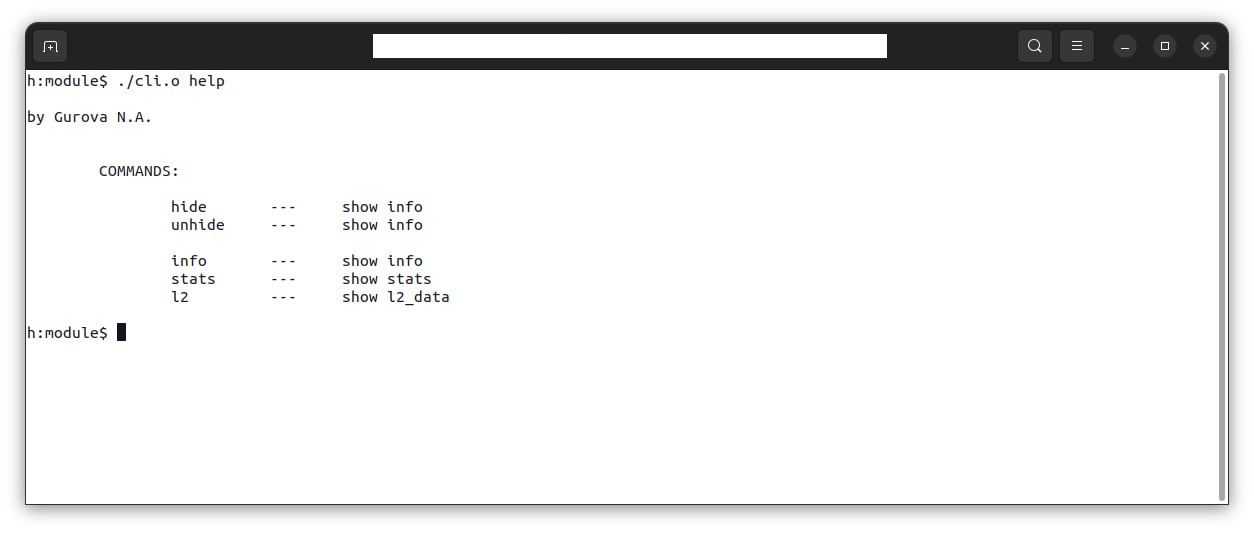
\includegraphics[width=0.95\textwidth]{inc/img/help.png}
 \caption{Вызов команды help}
 \label{img:help}
\end{figure}

\section{Видимость модуля}
Для скрытия модуля следует вызвать команду \textbf{hide}, а для обратного действия \textbf{unhide}. На рисунке~\ref{img:hide_unhide} демонстрируется следующее:

\begin{itemize}
\item[---] модуль загружен и виден в системе;
\item[---] вызвана команда hide;
\item[---] модуль не отображается при вызове команды lsmod;
\item[---] вызвана команда unhide;
\item[---] модуль обнаруживается при вызове команды lsmod.
\end{itemize}

\begin{figure}[hbtp]
 \centering
 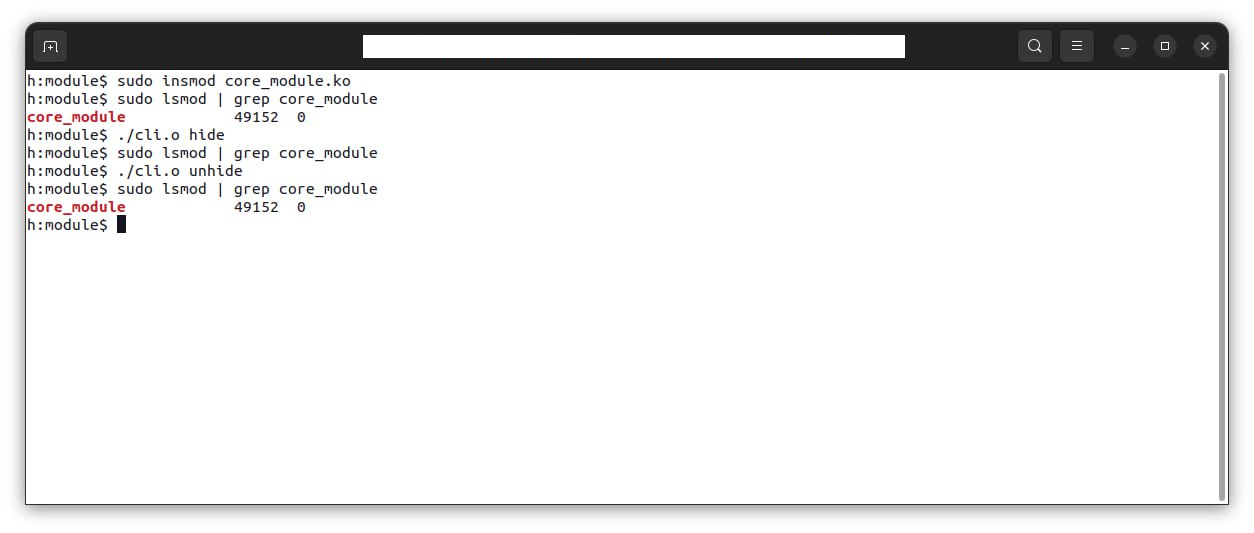
\includegraphics[width=0.95\textwidth]{inc/img/hide_unhide.png}
 \caption{Управление видимостью модуля}
 \label{img:hide_unhide}
\end{figure}

\section{Вывод статистики по работе модуля}
Для просмотра статистики по работе модуля предусмотрена команда \textbf{stats}. Эта команда позволяет просмотреть агрегированную статистику работы модуля: максимальная длина исторических данных, текущая длина исторических данных, текущая длина исторических данных (в секундах), количество критических периодов, первая временная метка возникновения критически активного периода, последняя временная метка возникновения критически активного периода.

На рисунке~\ref{img:stats} представлена демонстрация работы команды \textbf{stats}.   

\begin{figure}[hbtp]
 \centering
 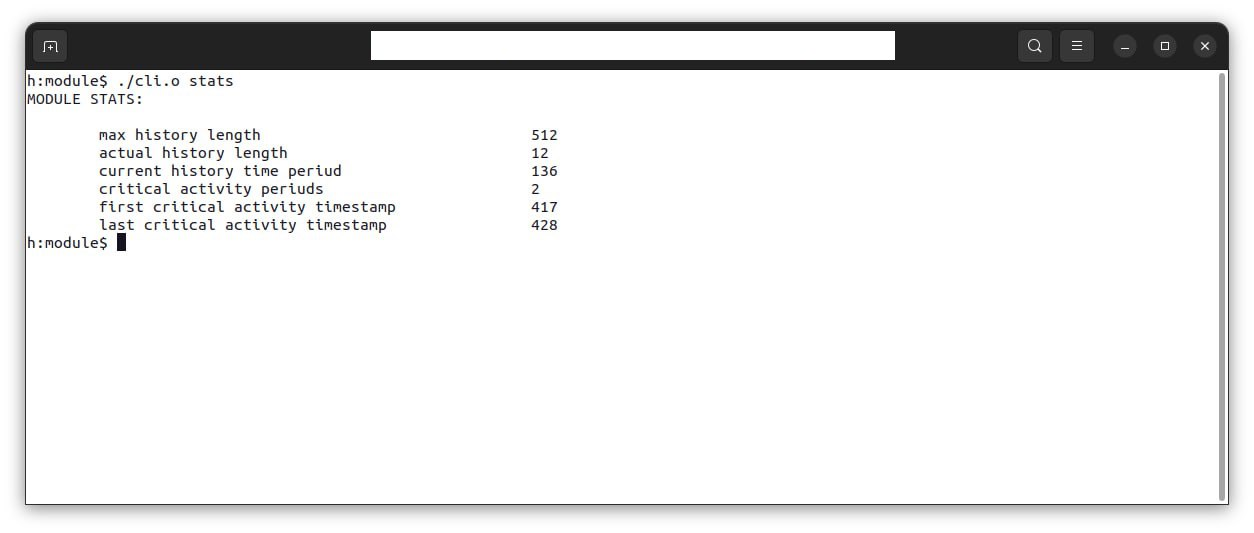
\includegraphics[width=0.95\textwidth]{inc/img/stats.jpg}
 \caption{Вывод статистики по работе модуля}
 \label{img:stats}
\end{figure}

\section{Просмотр исторических данных}
Для просмотра собранных исторических данных предусмотрена команда \textbf{l2}. Данная команда выводит собранные исторические данные в виде последовательности json-документов. Отчет о временном промежутке включает: временную метку периода, количество уникальных источников трафика, общее количество перехваченных пакетов, общий размер перехваченного трафика (в байтах), среднее количество перехваченных пакетов, максимальное количество перехваченных пакетов, средний размер перехваченных пакетов (в байтах), максимальный размер перехваченных пакетов (в байтах), флаг наличия аномалия, название аномального параметра.

На рисунке~\ref{img:l2} представлен результат выполнения команды \textbf{l2}.

\begin{figure}[hbtp]
 \centering
 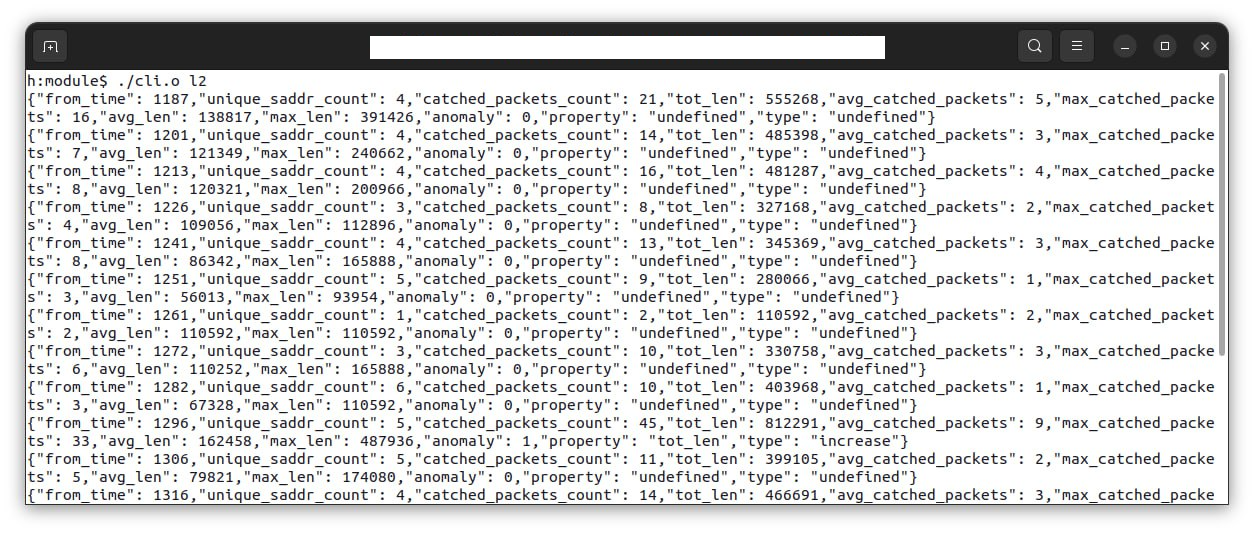
\includegraphics[width=0.95\textwidth]{inc/img/l2.png}
 \caption{Просмотр статистики}
 \label{img:l2}
\end{figure}

\section{Вывод}
В данном разделе была проведена демонстрация работы разработанного программного обеспечения.

В качестве результатов работы разработанного программного обеспечения приводятся изображения работы интерфейса командной строки.

Продемонстрированы: подсказка интерфейса командной строки, возможность изменения видимости загружаемого модуля ядра ОС Linux, возможность просмотра статистики работы загружаемого модуля для ОС Linux, возможность просмотра собранных исторических данных.

% ***************************************************************************

\chapter*{ЗАКЛЮЧЕНИЕ}
\addcontentsline{toc}{chapter}{ЗАКЛЮЧЕНИЕ}

В ходе выполнения курсовой работы был определен способ перехвата входящих и исходящих пакетов~---~путем регистрации функций перехвата с использованием библиотеки Netfilter. 

В качестве точек перехвата было решено использовать точку, которую проходят все исходящие пакеты (NF\_INET\_LOCAL\_IN).

Был разработан загружаемый модуль ядра ОС Linux, который осуществляет поиск атак во входящем сетевом трафике. Также был разработан интерфейс командной строки для управления разработанным загружаемым модулем для ядра ОС Linux. Предусмотрена возможность сокрытия модуля.

Продемонстрированы: подсказка интерфейса командной строки, возможность изменения видимости загружаемого модуля ядра ОС Linux, возможность просмотра статистики работы загружаемого модуля для ОС Linux, возможность просмотра собранных исторических данных.
\makebibliography

\chapter*{ПРИЛОЖЕНИЕ A}
\addcontentsline{toc}{chapter}{ПРИЛОЖЕНИЕ A}
\begin{lstlisting}[caption = {core\_module.h}]
#ifndef CORE_MODULE_H
#define CORE_MODULE_H


#define L2_DATA_DEV_PATH "/dev/cource_work_l2_data"
#define STATS_DEV_PATH "/dev/cource_work_stats"
#define CTRL_DEV_PATH "/dev/cource_work_ctrl"

enum command_type {
    UNDEFINED = 0,
    HIDE = 1,
    UNHIDE = 2,
};

struct command
{
    enum command_type type;
};

enum l2_property {
    L2_PROPERTY_UNDEFINED = 0,
    L2_PROPERTY_UNIQUE_SADDRS_COUNT = 1,
    L2_PROPERTY_CATCHED_PACKETS_COUNT = 2,
    L2_PROPERTY_TOT_LEN = 3,
    L2_PROPERTY_AVG_CATCHED_PACKETS = 4,
    L2_PROPERTY_MAX_CATCHED_PACKETS = 5,
    L2_PROPERTY_AVG_LEN = 6,
    L2_PROPERTY_MAX_LEN = 7,
    L2_PROPERTY_TOT_TCP = 8,
    L2_PROPERTY_TOT_SYN = 9,
};
enum l2_crit_behaviour_type {
    L2_CRIT_BEHAVIOUR_TYPE_UNDEFINED = 0,
    L2_CRIT_BEHAVIOUR_TYPE_INCREASE = 1,
    L2_CRIT_BEHAVIOUR_TYPE_FALL = 2,
};

struct l2_data_slice
{
    uint64_t from_time;
    uint32_t unique_saddr_count;
    uint32_t catched_packets_count;
    uint32_t tot_len;
    uint32_t avg_catched_packets;
    uint32_t max_catched_packets;
    uint32_t avg_len;
    uint32_t max_len;
    int crit_behaviour;
    enum l2_property property;
    enum l2_crit_behaviour_type type;
    uint32_t tot_tcp;
    uint32_t tot_syn;
};

struct module_stats
{
    uint32_t history_length;
    uint32_t current_history_length;
    uint64_t current_periud_ns;
    uint32_t crit_behaviour_count;
    uint64_t first_crit_behaviour_ns;
    uint64_t last_crit_behaviour_ns;
};

#endif //CORE_MODULE_H
\end{lstlisting}

\chapter*{ПРИЛОЖЕНИЕ Б}
\addcontentsline{toc}{chapter}{ПРИЛОЖЕНИЕ Б}
\begin{lstlisting}[caption = {core\_module.c}]
#include <linux/kernel.h>
#include <linux/module.h>
#include <linux/fs.h>
#include <linux/init.h> 
#include <linux/list.h>
#include <linux/slab.h>
#include <linux/cdev.h> 
#include <linux/device.h>
#include <linux/types.h>

#include <linux/netfilter_ipv4.h>
#include <linux/netfilter.h>
#include <linux/in.h>
#include <linux/ip.h>
#include <linux/tcp.h>
#include <linux/udp.h>

#include <linux/fcntl.h>
#include <linux/delay.h>
#include <linux/syscalls.h>

#include <linux/miscdevice.h>
#include <linux/stat.h>

#include <linux/string.h>
#include <linux/timekeeping.h>


#include "core_module.h"


#define MODULE_DMESG_PREFIX ">>>--------> "
#define DEVICE_L2_DATA_FNAME "cource_work_l2_data"
#define DEVICE_STATS_FNAME "cource_work_stats"
#define DEVICE_CTRL_FNAME "cource_work_ctrl"


#define IP_POS(ip, pos) (ip >> ((8 * (3 - pos))) & 0xFF)
#define SAME_ADDR(ip1, ip2) ((ip1 ^ ip2) == 0)

MODULE_LICENSE("GPL");
MODULE_AUTHOR("Gurova N.A.");

uint64_t dump_ns_periud = 10000000000;

#define FIRST_LAYER_TABLE_LENGTH 64
struct first_layer_schema {
    uint32_t unique_saddr;
    uint32_t catched_packets_count;
    uint32_t tot_len;
    uint32_t catched_tcp;
    uint32_t catched_syn;
};
struct first_layer_schema first_layer_table[FIRST_LAYER_TABLE_LENGTH];
size_t first_layer_table_next_index = 0;
uint64_t from_time = 0; // ns

#define SECOND_LAYER_TABLE_LENGTH 512
enum crit_behaviour_property {
    CRIT_BEHAVIOUR_PROPERTY_UNDEFINED = 0,
    CRIT_BEHAVIOUR_PROPERTY_UNIQUE_SADDRS_COUNT = 1,
    CRIT_BEHAVIOUR_PROPERTY_CATCHED_PACKETS_COUNT = 2,
    CRIT_BEHAVIOUR_PROPERTY_TOT_LEN = 3,
    CRIT_BEHAVIOUR_PROPERTY_AVG_CATCHED_PACKETS = 4,
    CRIT_BEHAVIOUR_PROPERTY_MAX_CATCHED_PACKETS = 5,
    CRIT_BEHAVIOUR_PROPERTY_AVG_LEN = 6,
    CRIT_BEHAVIOUR_PROPERTY_MAX_LEN = 7,
    CRIT_BEHAVIOUR_PROPERTY_TOT_TCP = 8,
    CRIT_BEHAVIOUR_PROPERTY_TOT_SYN = 9,
};
enum crit_behaviour_type {
    CRIT_BEHAVIOUR_TYPE_UNDEFINED = 0,
    CRIT_BEHAVIOUR_TYPE_INCREASE = 1,
    CRIT_BEHAVIOUR_TYPE_FALL = 2,
};
struct second_layer_schema {
    uint64_t from_time;
    uint32_t unique_saddr_count;
    uint32_t catched_packets_count;
    uint32_t tot_len;
    uint32_t avg_catched_packets;
    uint32_t max_catched_packets;
    uint32_t avg_len;
    uint32_t max_len;
    int crit_behaviour;
    enum crit_behaviour_property property;
    enum crit_behaviour_type type;
    uint32_t tot_tcp;
    uint32_t tot_syn;
};
struct second_layer_schema second_layer_table[SECOND_LAYER_TABLE_LENGTH];
size_t second_layer_table_next_index = 0;
size_t second_layer_table_read_index = 0;

struct second_layer_schema initial_vec = {
    .unique_saddr_count = 10,
    .catched_packets_count = 100,
    .tot_len = 1000000,
    .avg_catched_packets = 50,
    .max_catched_packets = 50,
    .avg_len = 300000,
    .max_len = 300000,
    .tot_tcp = 100,
    .tot_syn = 100,
};

int eps_percent = 30;

void inspect_last(void) {
    if (second_layer_table_next_index < 2) {
        return;
    }

    struct second_layer_schema avg_values = {
        .unique_saddr_count = 0,
        .catched_packets_count = 0,
        .tot_len = 0,
        .avg_catched_packets = 0,
        .max_catched_packets = 0,
        .avg_len = 0,
        .max_len = 0,
        .tot_tcp = 0,
        .tot_syn = 0,
    };

    for (int i = 0; i < second_layer_table_next_index - 1; i++) {
        avg_values.unique_saddr_count += second_layer_table[i].unique_saddr_count;
        avg_values.catched_packets_count += second_layer_table[i].catched_packets_count;
        avg_values.tot_len += second_layer_table[i].tot_len;
        avg_values.avg_catched_packets += second_layer_table[i].avg_catched_packets;
        avg_values.max_catched_packets += second_layer_table[i].max_catched_packets;
        avg_values.avg_len += second_layer_table[i].avg_len;
        avg_values.max_len += second_layer_table[i].max_len;
        avg_values.tot_tcp += second_layer_table[i].tot_tcp;
        avg_values.tot_syn += second_layer_table[i].tot_syn;
    }

    avg_values.unique_saddr_count /= (second_layer_table_next_index - 1);
    avg_values.catched_packets_count /= (second_layer_table_next_index - 1);
    avg_values.tot_len /= (second_layer_table_next_index - 1);
    avg_values.avg_catched_packets /= (second_layer_table_next_index - 1);
    avg_values.max_catched_packets /= (second_layer_table_next_index - 1);
    avg_values.avg_len /= (second_layer_table_next_index - 1);
    avg_values.max_len /= (second_layer_table_next_index - 1);
    avg_values.tot_tcp /= (second_layer_table_next_index - 1);
    avg_values.tot_syn /= (second_layer_table_next_index - 1);

    struct second_layer_schema last = second_layer_table[second_layer_table_next_index - 1];

    uint64_t limit;

    limit = avg_values.unique_saddr_count * (100 + eps_percent) / 100 + initial_vec.unique_saddr_count;
    if (last.unique_saddr_count > limit) {
        second_layer_table[second_layer_table_next_index - 1].crit_behaviour = 1;
        second_layer_table[second_layer_table_next_index - 1].property = CRIT_BEHAVIOUR_PROPERTY_UNIQUE_SADDRS_COUNT;
        second_layer_table[second_layer_table_next_index - 1].type = CRIT_BEHAVIOUR_TYPE_INCREASE;
        return;
    }

    limit = avg_values.catched_packets_count * (100 + eps_percent) / 100 + initial_vec.catched_packets_count;
    if (last.catched_packets_count > limit) {
        second_layer_table[second_layer_table_next_index - 1].crit_behaviour = 1;
        second_layer_table[second_layer_table_next_index - 1].property = CRIT_BEHAVIOUR_PROPERTY_CATCHED_PACKETS_COUNT;
        second_layer_table[second_layer_table_next_index - 1].type = CRIT_BEHAVIOUR_TYPE_INCREASE;
        return;
    }

    limit = avg_values.tot_len * (100 + eps_percent) / 100 + initial_vec.tot_len;
    if (last.tot_len > limit) {
        second_layer_table[second_layer_table_next_index - 1].crit_behaviour = 1;
        second_layer_table[second_layer_table_next_index - 1].property = CRIT_BEHAVIOUR_PROPERTY_TOT_LEN;
        second_layer_table[second_layer_table_next_index - 1].type = CRIT_BEHAVIOUR_TYPE_INCREASE;
        return;
    }

    limit = avg_values.avg_catched_packets * (100 + eps_percent) / 100 + initial_vec.avg_catched_packets;
    if (last.avg_catched_packets > limit) {
        second_layer_table[second_layer_table_next_index - 1].crit_behaviour = 1;
        second_layer_table[second_layer_table_next_index - 1].property = CRIT_BEHAVIOUR_PROPERTY_AVG_CATCHED_PACKETS;
        second_layer_table[second_layer_table_next_index - 1].type = CRIT_BEHAVIOUR_TYPE_INCREASE;
        return;
    }

    limit = avg_values.max_catched_packets * (100 + eps_percent) / 100 + initial_vec.max_catched_packets;
    if (last.max_catched_packets > limit) {
        second_layer_table[second_layer_table_next_index - 1].crit_behaviour = 1;
        second_layer_table[second_layer_table_next_index - 1].property = CRIT_BEHAVIOUR_PROPERTY_MAX_CATCHED_PACKETS;
        second_layer_table[second_layer_table_next_index - 1].type = CRIT_BEHAVIOUR_TYPE_INCREASE;
        return;
    }

    limit = avg_values.avg_len * (100 + eps_percent) / 100 + initial_vec.avg_len;
    if (last.avg_len > limit) {
        second_layer_table[second_layer_table_next_index - 1].crit_behaviour = 1;
        second_layer_table[second_layer_table_next_index - 1].property = CRIT_BEHAVIOUR_PROPERTY_AVG_LEN;
        second_layer_table[second_layer_table_next_index - 1].type = CRIT_BEHAVIOUR_TYPE_INCREASE;
        return;
    }

    limit = avg_values.max_len * (100 + eps_percent) / 100 + initial_vec.max_len;
    if (last.max_len > limit) {
        second_layer_table[second_layer_table_next_index - 1].crit_behaviour = 1;
        second_layer_table[second_layer_table_next_index - 1].property = CRIT_BEHAVIOUR_PROPERTY_MAX_LEN;
        second_layer_table[second_layer_table_next_index - 1].type = CRIT_BEHAVIOUR_TYPE_INCREASE;
        return;
    }

    limit = avg_values.tot_tcp * (100 + eps_percent) / 100 + initial_vec.tot_tcp;
    if (last.tot_tcp > limit) {
        second_layer_table[second_layer_table_next_index - 1].crit_behaviour = 1;
        second_layer_table[second_layer_table_next_index - 1].property = CRIT_BEHAVIOUR_PROPERTY_TOT_TCP;
        second_layer_table[second_layer_table_next_index - 1].type = CRIT_BEHAVIOUR_TYPE_INCREASE;
        return;
    }

    limit = avg_values.tot_syn * (100 + eps_percent) / 100 + initial_vec.tot_syn;
    if (last.tot_syn > limit) {
        second_layer_table[second_layer_table_next_index - 1].crit_behaviour = 1;
        second_layer_table[second_layer_table_next_index - 1].property = CRIT_BEHAVIOUR_PROPERTY_TOT_SYN;
        second_layer_table[second_layer_table_next_index - 1].type = CRIT_BEHAVIOUR_TYPE_INCREASE;
        return;
    }
}

void dump_first_layer_table(void) {
    if (second_layer_table_next_index >= SECOND_LAYER_TABLE_LENGTH) {
        for (int i = 0; i < SECOND_LAYER_TABLE_LENGTH - 1; i++) {
            second_layer_table[i] = second_layer_table[i + 1];
        }

        second_layer_table_next_index -= 1;
    }

    if (second_layer_table_next_index < SECOND_LAYER_TABLE_LENGTH) {
        uint32_t catched_packets_count = 0;
        uint32_t tot_len = 0;
        uint32_t avg_catched_packets = 0;
        uint32_t max_catched_packets = 0;
        uint32_t avg_len = 0;
        uint32_t max_len = 0;
        uint32_t tot_tcp = 0;
        uint32_t tot_syn = 0;

        for (int i = 0; i < first_layer_table_next_index; i++) {
            catched_packets_count += first_layer_table[i].catched_packets_count;
            tot_len += first_layer_table[i].tot_len;
            if (max_catched_packets < first_layer_table[i].catched_packets_count) { max_catched_packets = first_layer_table[i].catched_packets_count; }
            if (max_len < first_layer_table[i].tot_len) { max_len = first_layer_table[i].tot_len; }

            tot_tcp += first_layer_table[i].catched_tcp;
            tot_syn += first_layer_table[i].catched_syn;
        }

        avg_catched_packets = catched_packets_count / first_layer_table_next_index;
        avg_len = tot_len / first_layer_table_next_index;

        second_layer_table[second_layer_table_next_index].from_time = ktime_get_seconds();
        second_layer_table[second_layer_table_next_index]
            .unique_saddr_count = first_layer_table_next_index;
        second_layer_table[second_layer_table_next_index]
            .catched_packets_count = catched_packets_count;
        second_layer_table[second_layer_table_next_index]
            .tot_len = tot_len;
        second_layer_table[second_layer_table_next_index]
            .avg_catched_packets = avg_catched_packets;
        second_layer_table[second_layer_table_next_index]
            .max_catched_packets = max_catched_packets;
        second_layer_table[second_layer_table_next_index]
            .avg_len = avg_len;
        second_layer_table[second_layer_table_next_index]
            .max_len = max_len;

        second_layer_table[second_layer_table_next_index]
            .crit_behaviour = 0;
        second_layer_table[second_layer_table_next_index]
            .property = CRIT_BEHAVIOUR_PROPERTY_UNDEFINED;
        second_layer_table[second_layer_table_next_index]
            .type = CRIT_BEHAVIOUR_TYPE_UNDEFINED;

        second_layer_table[second_layer_table_next_index]
            .tot_tcp = tot_tcp;
        second_layer_table[second_layer_table_next_index]
            .tot_syn = tot_syn;        

        first_layer_table_next_index = 0;
        second_layer_table_next_index += 1;

        inspect_last();
    }
}

void add_packet_info(uint32_t saddr, uint32_t tot_len, uint32_t is_tcp, uint32_t is_syn) {

    if (ktime_get_ns() - from_time > dump_ns_periud) {
        if (from_time != 0) dump_first_layer_table();

        from_time = ktime_get_ns();
    }

    int records_found = 0;

    for (int i = 0; i < first_layer_table_next_index; i++) {
        if (first_layer_table[i].unique_saddr == saddr) {
            records_found = 1;

            first_layer_table[i].catched_packets_count += 1;
            first_layer_table[i].tot_len += tot_len;

            if (is_tcp) first_layer_table[i].catched_tcp += 1;
            if (is_syn) first_layer_table[i].catched_syn += 1;

            break;
        }
    }

    if (records_found != 1 && first_layer_table_next_index < FIRST_LAYER_TABLE_LENGTH) {
        first_layer_table[first_layer_table_next_index]
            .unique_saddr = saddr;
        first_layer_table[first_layer_table_next_index]
            .catched_packets_count = 1;
        first_layer_table[first_layer_table_next_index]
            .tot_len = tot_len;

        if (is_tcp) {
            first_layer_table[first_layer_table_next_index]
                .catched_tcp = 1;
        } else {
            first_layer_table[first_layer_table_next_index]
                .catched_tcp = 0;
        }

        if (is_syn) {
            first_layer_table[first_layer_table_next_index]
                .catched_syn= 1;
        } else {
            first_layer_table[first_layer_table_next_index]
                .catched_syn= 0;
        }

        first_layer_table_next_index += 1;
    }
}


static unsigned int catch_traffic(void *priv, struct sk_buff *skb, const struct nf_hook_state *state)
{
    struct iphdr *iph;  /* An IPv4 packet header */
    struct tcphdr *tcph; /* An TCP packet header */
    uint32_t saddr;
    uint32_t tot_len;
    uint32_t is_tcp = 0;
    uint32_t is_syn = 0;

    if (!skb) return NF_ACCEPT;

    iph = (struct iphdr *)skb_network_header(skb);
    if (iph == NULL) return NF_ACCEPT;

    saddr = iph->saddr;
    tot_len = iph->tot_len;

    if (iph->protocol == IPPROTO_TCP) {
        tcph = (struct tcphdr *)(skb_transport_header(skb));
        is_tcp = 1;
        if (tcph->syn) is_syn = 1;
    }

    add_packet_info(saddr, tot_len, is_tcp, is_syn);

    return NF_ACCEPT;   /* the packet passes, continue iterations */
}

static struct nf_hook_ops module_hook_ops = 
{
    .hook = catch_traffic,
    .pf = PF_INET,
    .hooknum = NF_INET_LOCAL_IN,
    .priority = NF_IP_PRI_FIRST
};

// hide && unhide

struct list_head *module_prev;
int flag_hidden = 0;

void hide(void) {
    if (flag_hidden)
        return;

    module_prev = THIS_MODULE->list.prev;
    list_del(&THIS_MODULE->list);
    flag_hidden = 1;

    printk("module was hidden");
}

void unhide(void) {
    if (!flag_hidden)
        return;

    list_add(&THIS_MODULE->list, module_prev);
    flag_hidden = 0;

    printk("module was exposed");
} 

// misc devices description

ssize_t write_stub(struct file *filp, const char __user *buff, size_t count, loff_t *f_pos) { return 0; }
ssize_t read_stub(struct file *filp, char __user *buff, size_t count, loff_t *f_pos) { return 0; }
int open_stub(struct inode *inode, struct file *file) { return 0; }
int release_stub(struct inode *inode, struct file *file) { return 0; }

ssize_t read_l2_data(struct file *filp, char __user *buff, size_t count, loff_t *f_pos) {
    if (count != sizeof(struct l2_data_slice)) {
        printk(MODULE_DMESG_PREFIX "[ERROR] invalid count");
        return 0;
    }
    
    if (second_layer_table_read_index >= second_layer_table_next_index) {
        second_layer_table_read_index = 0;
        return 0;
    }

    struct l2_data_slice l2_ds = {
        .from_time = second_layer_table[second_layer_table_read_index]
            .from_time,
        .unique_saddr_count = second_layer_table[second_layer_table_read_index]
            .unique_saddr_count,
        .catched_packets_count = second_layer_table[second_layer_table_read_index]
            .catched_packets_count,
        .tot_len = second_layer_table[second_layer_table_read_index]
            .tot_len,
        .avg_catched_packets = second_layer_table[second_layer_table_read_index]
            .avg_catched_packets,
        .max_catched_packets = second_layer_table[second_layer_table_read_index]
            .max_catched_packets,
        .avg_len = second_layer_table[second_layer_table_read_index]
            .avg_len,
        .max_len = second_layer_table[second_layer_table_read_index]
            .max_len,
        .crit_behaviour = second_layer_table[second_layer_table_read_index]
            .crit_behaviour,
        .property = second_layer_table[second_layer_table_read_index]
            .property,
        .type = second_layer_table[second_layer_table_read_index]
            .type,
        .tot_tcp = second_layer_table[second_layer_table_read_index]
            .tot_tcp,
        .tot_syn = second_layer_table[second_layer_table_read_index]
            .tot_syn,
    };

    if (copy_to_user(buff, (char *) &l2_ds, sizeof(struct l2_data_slice)))
    {
        printk(MODULE_DMESG_PREFIX "[ERROR] copy_to_user error");
        return 0;
    }

    second_layer_table_read_index += 1;

    return sizeof(struct l2_data_slice);
}

ssize_t read_stats(struct file *filp, char __user *buff, size_t count, loff_t *f_pos) {
    if (count != sizeof(struct module_stats)) {
        printk(MODULE_DMESG_PREFIX "[ERROR] invalid count");
        return 0;
    }

    uint32_t history_length = SECOND_LAYER_TABLE_LENGTH;
    uint32_t current_history_length = second_layer_table_next_index;
    uint64_t current_periud_ns = 0;
    uint32_t crit_behaviour_count = 0;
    uint64_t first_crit_behaviour_ns = 0;
    uint64_t last_crit_behaviour_ns = 0;

    for (int i = 0; i < second_layer_table_next_index; i++) {
        if (second_layer_table[i].crit_behaviour > 0) {
            crit_behaviour_count += 1;
            if (first_crit_behaviour_ns == 0) {
                first_crit_behaviour_ns = second_layer_table[i].from_time;
            }
            last_crit_behaviour_ns = second_layer_table[i].from_time;
        }
    }

    uint64_t per_start = 0, per_finish = 0;
    if (second_layer_table_next_index > 0) {
        per_start = second_layer_table[0].from_time;
        per_finish = second_layer_table[second_layer_table_next_index - 1].from_time;
        // printk(MODULE_DMESG_PREFIX "%lld %lld", per_start, per_finish);
    }
    current_periud_ns = per_finish - per_start;

    struct module_stats stats = {
        .history_length = history_length,
        .current_history_length = current_history_length,
        .current_periud_ns = current_periud_ns,
        .crit_behaviour_count = crit_behaviour_count,
        .first_crit_behaviour_ns = first_crit_behaviour_ns,
        .last_crit_behaviour_ns = last_crit_behaviour_ns,
    };

    if (copy_to_user(buff, (char *) &stats, sizeof(struct module_stats)))
    {
        printk(MODULE_DMESG_PREFIX "[ERROR] copy_to_user error");
        return 0;
    }

    return sizeof(struct module_stats);
}

ssize_t write_command(struct file *filp, const char __user *buff, size_t count, loff_t *f_pos) 
{
    struct command cmd;

    if (count != sizeof(struct command))
    {
        printk(MODULE_DMESG_PREFIX "[ERROR] incorrect command");
        return 0;
    }

    if (copy_from_user(&cmd, buff, sizeof(struct command)))
    {
        printk(MODULE_DMESG_PREFIX "[ERROR] copy_from_user error");
        return 0;
    }

    if (cmd.type == HIDE) {
        hide();
    }

    if (cmd.type == UNHIDE) {
        unhide();
    }

    return 0; 
}

static struct file_operations l2_data_fops = {
    .owner = THIS_MODULE,
    .read = read_l2_data,
    .write = write_stub,
    .open = open_stub,
    .release = release_stub,
};

static struct file_operations stats_fops = {
    .owner = THIS_MODULE,
    .read = read_stats,
    .write = write_stub,
    .open = open_stub,
    .release = release_stub,
};

static struct file_operations ctrl_fops = {
    .owner = THIS_MODULE,
    .read = read_stub,
    .write = write_command,
    .open = open_stub,
    .release = release_stub,
};

struct miscdevice dev_l2_data = {
    .minor = MISC_DYNAMIC_MINOR,
    .name = DEVICE_L2_DATA_FNAME,
    .fops = &l2_data_fops,
    .mode = S_IRWXU | S_IWGRP | S_IWOTH | S_IROTH,
};

struct miscdevice dev_stats = {
    .minor = MISC_DYNAMIC_MINOR,
    .name = DEVICE_STATS_FNAME,
    .fops = &stats_fops,
    .mode = S_IRWXU | S_IWGRP | S_IWOTH | S_IROTH,
};

struct miscdevice dev_ctrl = {
    .minor = MISC_DYNAMIC_MINOR,
    .name = DEVICE_CTRL_FNAME,
    .fops = &ctrl_fops,
    .mode = S_IRWXU | S_IWGRP | S_IWOTH | S_IROTH,
};

static int __init my_module_init(void) {
    int rc = 0;

    nf_register_net_hook(&init_net, &module_hook_ops);

    rc = misc_register(&dev_l2_data);
    if (rc)
    {
        printk(MODULE_DMESG_PREFIX "[ERROR] registration was failed");
        return rc;
    }

    rc = misc_register(&dev_stats);
    if (rc)
    {
        printk(MODULE_DMESG_PREFIX "[ERROR] registration was failed");
        return rc;
    }

    rc = misc_register(&dev_ctrl);
    if (rc)
    {
        printk(MODULE_DMESG_PREFIX "[ERROR] registration was failed");
        return rc;
    }

    printk(MODULE_DMESG_PREFIX "module was loaded");

    return 0;
}

static void __exit my_module_exit(void) {

    nf_unregister_net_hook(&init_net, &module_hook_ops);

    misc_deregister(&dev_l2_data);
    misc_deregister(&dev_stats);
    misc_deregister(&dev_ctrl);

    printk(MODULE_DMESG_PREFIX "module was unloaded\n");
}

module_init(my_module_init);
module_exit(my_module_exit);
\end{lstlisting}

\chapter*{ПРИЛОЖЕНИЕ В}
\addcontentsline{toc}{chapter}{ПРИЛОЖЕНИЕ В}
\begin{lstlisting}[caption = {cli.c}]
#include <stdio.h>
#include <stdlib.h>
#include <getopt.h>
#include <arpa/inet.h>
#include <netdb.h>
#include <limits.h>
#include <string.h>
#include <fcntl.h>

#include <unistd.h>

#include "core_module.h"

#define PROPERTY_COUNT 10
enum l2_property properties[] = {L2_PROPERTY_UNDEFINED, L2_PROPERTY_UNIQUE_SADDRS_COUNT, L2_PROPERTY_CATCHED_PACKETS_COUNT, L2_PROPERTY_TOT_LEN, 
    L2_PROPERTY_AVG_CATCHED_PACKETS, L2_PROPERTY_MAX_CATCHED_PACKETS, L2_PROPERTY_AVG_LEN, L2_PROPERTY_MAX_LEN, L2_PROPERTY_TOT_TCP, L2_PROPERTY_TOT_SYN};
char *property_names[] = {"undefined", "saddr_count", "catched_packet_count", "tot_len", "avg_catched_packets",
 "max_catched_packets", "avg_len", "max_len", "tot_tcp", "tot_syn"};
char *get_property_name(enum l2_property prop) {
    for (int i = 0; i < PROPERTY_COUNT; i++) {
        if (properties[i] == prop) {
            return property_names[i];
        }
    }
    return property_names[0];
}

#define crit_behaviour_TYPE_COUNT 3
enum l2_crit_behaviour_type crit_behaviour_types[] = {L2_CRIT_BEHAVIOUR_TYPE_UNDEFINED, L2_CRIT_BEHAVIOUR_TYPE_INCREASE, L2_CRIT_BEHAVIOUR_TYPE_FALL};
char *crit_behaviour_type_names[] = {"undefined", "increase", "fall"};
char *get_crit_behaviour_type_name(enum l2_crit_behaviour_type at) {
    for (int i = 0; i < crit_behaviour_TYPE_COUNT; i++) {
        if (crit_behaviour_types[i] == at) {
            return crit_behaviour_type_names[i];
        }
    }
    return crit_behaviour_type_names[0];
}

void print_info(void) {
    printf(
        "\nby Gurova N.A.\n\n\n"
        "\tCOMMANDS:\n\n"
        "\t\thide       ---     hide\n"
        "\t\tunhide     ---     unhide\n\n"
        "\t\tinfo       ---     show info\n"
        "\t\tstats      ---     show stats\n"
        "\t\tl2         ---     show l2_data\n\n"
    );
}

void print_l2_data_slice(struct l2_data_slice *l2_ds) {
    printf("{"
    "\"from_time\": %ld,"
    "\"unique_saddr_count\": %d,"
    "\"catched_packets_count\": %d,"
    "\"tot_len\": %d,"
    "\"avg_catched_packets\": %d,"
    "\"max_catched_packets\": %d,"
    "\"avg_len\": %d,"
    "\"max_len\": %d,"
    "\"crit\": %d,"
    "\"property\": \"%s\","
    "\"crit_type\": \"%s\","
    "\"tot_tcp\": \"%d\","
    "\"tot_syn\": \"%d\""
    "}\n", l2_ds->from_time, l2_ds->unique_saddr_count, l2_ds->catched_packets_count,
    l2_ds->tot_len, l2_ds->avg_catched_packets, l2_ds->max_catched_packets, l2_ds->avg_len,
    l2_ds->max_len, l2_ds->crit_behaviour, get_property_name(l2_ds->property), get_crit_behaviour_type_name(l2_ds->type),
    l2_ds->tot_tcp, l2_ds->tot_syn);
}

int show_l2_data()
{
    struct l2_data_slice ds;
    int rb;

    int fd = open(L2_DATA_DEV_PATH, O_RDONLY);
    if (fd < 0) return 1;

    size_t l2_ds_size = sizeof(struct l2_data_slice);

    while ((rb = read(fd, &ds, l2_ds_size)) > 0) {
        if (rb != l2_ds_size) break;

        print_l2_data_slice(&ds);
	}

    close(fd);

    return 0;
}

int show_stats()
{
    struct module_stats stats;
    int rb;

    int fd = open(STATS_DEV_PATH, O_RDONLY);
    if (fd < 0) return 1;

    size_t stats_size = sizeof(struct module_stats);

    if (read(fd, &stats, stats_size) != stats_size) {
        close(fd);
        return 1;
    }

    close(fd);

    printf(
        "MODULE STATS:\n\n"
        "\tmax history length\t\t\t\t%d\n"
        "\tactual history length\t\t\t\t%d\n"
        "\tcurrent history time periud\t\t\t%ld\n"
        "\tcritical activity periuds\t\t\t%d\n"
        "\tfirst critical activity timestamp\t\t%ld\n"
        "\tlast critical activity timestamp\t\t%ld\n",
        stats.history_length, stats.current_history_length, stats.current_periud_ns,
        stats.crit_behaviour_count, stats.first_crit_behaviour_ns, stats.last_crit_behaviour_ns
    );

    return 0;
}

void hide_unhide(int make_hidden) {
    struct command cmd;
    if (make_hidden == 1) {
        cmd.type = HIDE;
    } else {
        cmd.type = UNHIDE;
    }

    int fd = open(CTRL_DEV_PATH, O_WRONLY | O_APPEND);
    if (fd < 0) return;

    write(fd, &cmd, sizeof(struct command));

    close(fd);
}

int main(int argc, char *argv[])
{
    if (argc != 2) {
        print_info();
        return 1;
    }

    if (!strcmp(argv[1], "info")) {
        print_info();
        return 0;
    }

    if (!strcmp(argv[1], "stats")) {
        return show_stats();
    }

    if (!strcmp(argv[1], "l2")) {
        return show_l2_data();
    }

    if (!strcmp(argv[1], "hide")) {
        hide_unhide(1);
        return 0;
    }

    if (!strcmp(argv[1], "unhide")) {
        hide_unhide(0);
        return 0;
    }

    print_info();
    return 1;
}
\end{lstlisting}

\chapter*{ПРИЛОЖЕНИЕ Г}
\addcontentsline{toc}{chapter}{ПРИЛОЖЕНИЕ Г}
\begin{lstlisting}[caption = {Makefile}]
obj-m += core_module.o

all: cli.o core_module.o

cli.o: cli.c core_module.h
	gcc -o cli.o cli.c	

core_module.o: core_module.c
	make -C /lib/modules/$(shell uname -r)/build M=$(PWD) modules

clean:
	rm -rf cli *.o
	make -C /lib/modules/$(shell uname -r)/build M=$(PWD) clean
\end{lstlisting}


\end{document}


